% This is a part of the Rmarkdown thesis template for Statistics at Macquarie University (MQ)
% Created by Thomas Fung & Justin Wishart (MQ) (04 June 2018). 

% Most of the work for the document class was done by Sam Noble (SN), as well as this
% template. Later comments etc. by Ben Salzberg (BTS). Additional
% restructuring and APA support by Jess Youngberg (JY).

% See http://web.reed.edu/cis/help/latex.html for help. There are a
% great bunch of help pages there, with notes on
% getting started, bibtex, etc. Go there and read it if you're not
% already familiar with LaTeX.
%
% Any line that starts with a percent symbol is a comment.
% They won't show up in the document, and are useful for notes
% to yourself and explaining commands.
% Commenting also removes a line from the document;
% very handy for troubleshooting problems. -BTS

% As far as I know, this follows the requirements laid out in
% the 2002-2003 Senior Handbook. Ask a librarian to check the
% document before binding. -SN

%%
%% Preamble
%%
% \documentclass{<something>} must begin each LaTeX document
\documentclass[12pt,twoside, a4paper]{reedthesis}
% Packages are extensions to the basic LaTeX functions. Whatever you
% want to typeset, there is probably a package out there for it.
% Chemistry (chemtex), screenplays, you name it.
% Check out CTAN to see: http://www.ctan.org/
%%
\usepackage{graphicx,latexsym}
\usepackage{amsmath}
\usepackage{amssymb,amsthm}
\usepackage{longtable,booktabs,setspace}
\usepackage{chemarr} %% Useful for one reaction arrow, useless if you're not a chem major
\usepackage[hyphens]{url}
% Added by CII
\usepackage{hyperref}
\usepackage{lmodern}
\usepackage{float}
\floatplacement{figure}{H}
% End of CII addition
\usepackage{rotating}
\usepackage[top=1.5cm, bottom=2.0cm, inner=3.5cm, outer=2.0cm, includehead]{geometry}
% Next line commented out by CII
%%% \usepackage{natbib}
% Comment out the natbib line above and uncomment the following two lines to use the new
% biblatex-chicago style, for Chicago A. Also make some changes at the end where the
% bibliography is included.
%\usepackage{biblatex-chicago}
%\bibliography{thesis}

\renewcommand{\baselinestretch}{1.5}%
% Added by CII (Thanks, Hadley!)
% Use ref for internal links
\renewcommand{\hyperref}[2][???]{\autoref{#1}}
\def\chapterautorefname{Chapter}
\def\sectionautorefname{Section}
\def\subsectionautorefname{Subsection}
% End of CII addition

% Added by CII
\usepackage{caption}
\captionsetup{width=5in}
% End of CII addition

% \usepackage{times} % other fonts are available like times, bookman, charter, palatino

% Syntax highlighting #22
  \usepackage{color}
  \usepackage{fancyvrb}
  \newcommand{\VerbBar}{|}
  \newcommand{\VERB}{\Verb[commandchars=\\\{\}]}
  \DefineVerbatimEnvironment{Highlighting}{Verbatim}{commandchars=\\\{\}}
  % Add ',fontsize=\small' for more characters per line
  \newenvironment{Shaded}{}{}
  \newcommand{\AlertTok}[1]{\textcolor[rgb]{1.00,0.00,0.00}{\textbf{#1}}}
  \newcommand{\AnnotationTok}[1]{\textcolor[rgb]{0.38,0.63,0.69}{\textbf{\textit{#1}}}}
  \newcommand{\AttributeTok}[1]{\textcolor[rgb]{0.49,0.56,0.16}{#1}}
  \newcommand{\BaseNTok}[1]{\textcolor[rgb]{0.25,0.63,0.44}{#1}}
  \newcommand{\BuiltInTok}[1]{#1}
  \newcommand{\CharTok}[1]{\textcolor[rgb]{0.25,0.44,0.63}{#1}}
  \newcommand{\CommentTok}[1]{\textcolor[rgb]{0.38,0.63,0.69}{\textit{#1}}}
  \newcommand{\CommentVarTok}[1]{\textcolor[rgb]{0.38,0.63,0.69}{\textbf{\textit{#1}}}}
  \newcommand{\ConstantTok}[1]{\textcolor[rgb]{0.53,0.00,0.00}{#1}}
  \newcommand{\ControlFlowTok}[1]{\textcolor[rgb]{0.00,0.44,0.13}{\textbf{#1}}}
  \newcommand{\DataTypeTok}[1]{\textcolor[rgb]{0.56,0.13,0.00}{#1}}
  \newcommand{\DecValTok}[1]{\textcolor[rgb]{0.25,0.63,0.44}{#1}}
  \newcommand{\DocumentationTok}[1]{\textcolor[rgb]{0.73,0.13,0.13}{\textit{#1}}}
  \newcommand{\ErrorTok}[1]{\textcolor[rgb]{1.00,0.00,0.00}{\textbf{#1}}}
  \newcommand{\ExtensionTok}[1]{#1}
  \newcommand{\FloatTok}[1]{\textcolor[rgb]{0.25,0.63,0.44}{#1}}
  \newcommand{\FunctionTok}[1]{\textcolor[rgb]{0.02,0.16,0.49}{#1}}
  \newcommand{\ImportTok}[1]{#1}
  \newcommand{\InformationTok}[1]{\textcolor[rgb]{0.38,0.63,0.69}{\textbf{\textit{#1}}}}
  \newcommand{\KeywordTok}[1]{\textcolor[rgb]{0.00,0.44,0.13}{\textbf{#1}}}
  \newcommand{\NormalTok}[1]{#1}
  \newcommand{\OperatorTok}[1]{\textcolor[rgb]{0.40,0.40,0.40}{#1}}
  \newcommand{\OtherTok}[1]{\textcolor[rgb]{0.00,0.44,0.13}{#1}}
  \newcommand{\PreprocessorTok}[1]{\textcolor[rgb]{0.74,0.48,0.00}{#1}}
  \newcommand{\RegionMarkerTok}[1]{#1}
  \newcommand{\SpecialCharTok}[1]{\textcolor[rgb]{0.25,0.44,0.63}{#1}}
  \newcommand{\SpecialStringTok}[1]{\textcolor[rgb]{0.73,0.40,0.53}{#1}}
  \newcommand{\StringTok}[1]{\textcolor[rgb]{0.25,0.44,0.63}{#1}}
  \newcommand{\VariableTok}[1]{\textcolor[rgb]{0.10,0.09,0.49}{#1}}
  \newcommand{\VerbatimStringTok}[1]{\textcolor[rgb]{0.25,0.44,0.63}{#1}}
  \newcommand{\WarningTok}[1]{\textcolor[rgb]{0.38,0.63,0.69}{\textbf{\textit{#1}}}}

% To pass between YAML and LaTeX the dollar signs are added by CII
\title{Title: Comparing numerical performance of second generation wavelets and the nonparametric estimators in random design regression models}
\author{Mohammadhossein Aberoumand}
% The month and year that you submit your FINAL draft TO THE LIBRARY (May or December)
\date{June}
\division{}
\advisor{}
\institution{}
\degree{STAT825: Statistical Project}
%If you have two advisors for some reason, you can use the following
% Uncommented out by CII
% End of CII addition

%%% Remember to use the correct department!
\department{Statistics}
% if you're writing a thesis in an interdisciplinary major,
% uncomment the line below and change the text as appropriate.
% check the Senior Handbook if unsure.
%\thedivisionof{The Established Interdisciplinary Committee for}
% if you want the approval page to say "Approved for the Committee",
% uncomment the next line
%\approvedforthe{Committee}

% Added by CII
%%% Copied from knitr
%% maxwidth is the original width if it's less than linewidth
%% otherwise use linewidth (to make sure the graphics do not exceed the margin)
\makeatletter
\def\maxwidth{ %
  \ifdim\Gin@nat@width>\linewidth
    \linewidth
  \else
    \Gin@nat@width
  \fi
}
\makeatother

\renewcommand{\contentsname}{Table of Contents}
% End of CII addition

\setlength{\parskip}{0pt}

% Added by CII

\providecommand{\tightlist}{%
  \setlength{\itemsep}{0pt}\setlength{\parskip}{0pt}}

\Acknowledgements{
I would like to express my sincere gratitude to my supervisor Dr.~Justin Wishart for his help, support and patience for my Statistical project.
}

\Dedication{
This project is wholeheartedly dedicated to my family who have continuously supported me spiritually, emotionally and economically through my studies.
To my friends whose love and kindness has given me the energy and courage to work hard and finish my studies.
}



\LOP{ \doublespace
\begin{itemize}
\tightlist
\item
  insert author list \emph{insert paper title}. (submitted to insert journal name)
\item
  insert author list \emph{insert paper title}. insert journal name \textbf{insert volume number}, insert article or page number (insert year)
\end{itemize}
}

\Abstract{
Since wavelet methods were introduced three decades ago they have captured the attention of scientists in different areas. In the discipline of statistics, these methods have been implemented in different areas such as nonparametric regression, time series analysis and image denoising. In this project we have compared the relatively new second generation wavelet method with the first generation method and some commonly used nonparametric methods. We have tested these methods on non-equally-spaced grids and recorded the MSEs and MAEs. Based on the results of this project, the second generation wavelet method performs as well as the common nonparametric methods and is substantially better than the first generation in terms of error.
}

% End of CII addition
%%
%% End Preamble
%%
%
\begin{document}

% Everything below added by CII
  \maketitle


\frontmatter % this stuff will be roman-numbered
\pagestyle{headings} % this removes page numbers from the frontmatter
  \begin{acknowledgements}
    I would like to express my sincere gratitude to my supervisor Dr.~Justin Wishart for his help, support and patience for my Statistical project.
  \end{acknowledgements}
  \begin{abstract}
    Since wavelet methods were introduced three decades ago they have captured the attention of scientists in different areas. In the discipline of statistics, these methods have been implemented in different areas such as nonparametric regression, time series analysis and image denoising. In this project we have compared the relatively new second generation wavelet method with the first generation method and some commonly used nonparametric methods. We have tested these methods on non-equally-spaced grids and recorded the MSEs and MAEs. Based on the results of this project, the second generation wavelet method performs as well as the common nonparametric methods and is substantially better than the first generation in terms of error.
  \end{abstract}



  \hypersetup{linkcolor=black}
  \setcounter{tocdepth}{2}
  \tableofcontents




  \begin{dedication}
    This project is wholeheartedly dedicated to my family who have continuously supported me spiritually, emotionally and economically through my studies.
    To my friends whose love and kindness has given me the energy and courage to work hard and finish my studies.
  \end{dedication}
\mainmatter % here the regular arabic numbering starts
\pagestyle{fancyplain} % turns page numbering back on

\hypertarget{introduction}{%
\chapter{Introduction}\label{introduction}}

One of the most important topics in statistics is to model the mean value of response variable and linear statistical model are a classical tool to do so. Due to their simplistic nature, these family of models have been at the centre of attention for a long time. These models define a relationship between a response variable \(Y\) and a set of independent variable \(X_1,X_2,\dots,X_k\) such as the following:
\[Y=\beta_0+\beta_1X_1+\epsilon\]
\[\epsilon\sim N(0,1)\]
where \(\beta_0,\beta_1\) unknown parameter that we wish to estimate. Linear regression are discussed in more details in(Wackerly, Mendenhall, \& Scheaffer, 2014). Although, these models are based on linear relationships between variables, there will e many cases where we wish to investigate nonlinear relationships between the response and an independent variable. The general form of the model corresponds to it is the following:
\begin{equation}
Y=f(X)+\epsilon,\quad \epsilon\sim N(0,1)
\label{eq:reg}
\end{equation}
In equation \eqref{eq:reg} function \(f \in C^r\) which mean its derivatives exist till order \(r\) and it is bounded. When the relationship is nonlinear simple linear regression is not good choice because it is linear in nature and therefore not very flexible and although it will a have relatively small variance, its bias will be considerably large. Therefore, in chapter 2, we will briefly discuss some \emph{nonparametric methods} that can be used to find \(f\) such as \emph{Kernel smoothing}, \emph{Splines} and \emph{Wavelet methods} these method are more flexible compared to simple linear regression and will be less biased and by tuning their hyper parameters correctly we can avoid over-fitting. For instance, choice of bandwidth for \emph{Kernel smoothing} and number of knots for \emph{Spline} are crucial to get a good fit for the data. In this project we wish to compare first and second generation of \emph{wavelet method} with two other class of estimators mentioned above. The \emph{First generation wavelet method} are known to be applicable to the equally spaced grid However, They are not equally effective in the non equally spaced grid case due to its reliance on Fourier transformation. Since data-sets with non equally spaced grid are common in the real world cases over the past years a newly methods called \emph{second generation wavelet} method has been developed by scientists which can handle a non equally spaced grid. This algorithm benefits from a framework called \emph{lifting scheme} which does not rely on Fourier transformation. The second generation has been tested on real data-sets in (Hamilton, Nunes, Knight, \& Fryzlewicz, 2018). However, no comparison has been made between first and second generation wavelet method on a non equally spaced grid data. In this project we wish to put these methods to the test in numerous scenarios.

In chapter three, we will discuss the methods to simulated the data from a non equally space grid. To create a non equally spaced grid we will use a \emph{random design model}. In general, if in \eqref{eq:reg} only responses\(Y_1,\dots,Y_N\) are treated as random and the sample \(X_1,\dots,X_N\) treated to be fixed values this is called a \emph{fixed design}. In contrast, if \((X_1,Y_1),\dots,(X_N,Y_N)\) considered to be random pairs this is called \emph{random design}(Hsu, Kakade, \& Zhang, 2011). For demonstration purposes we will represent some graph of basic function and signals and the estimated curved by different methods.

In chapter four, we wish to compare these estimators by Mean square error and Mean absolute error. we will present the results of the simulations. Three type of grid will be generated from uniform, left skewed and right-skewed distributions. This is important due to nonsymmetric shape of the signals which will result in different amount of variation along the domain. In addition we will change the amount of noise added each time by changing the signal to noise ratio.

The preface pretty much says it all.

\par

Second paragraph of abstract starts here.

\hypertarget{non-parametric-regression}{%
\chapter{Non-parametric regression}\label{non-parametric-regression}}

In this chapter we will discuss different ideas and methods for nonparametric regression (Martinez \& Martinez, 2007) but before explaining the nonparametric methods we will recall the linear regression model this will help us have a better understanding of different approaches to this problem. A refinement of the previous linear regression model that could move in nonlinear patterns could be a ploynomial regression:
\begin{equation}
Y_{i}=\beta_{0}+\beta_{1}X+\beta_{2}X^{2}+...+\beta_{p}X^{p}+\epsilon, \quad p \in\mathbb{N}
 \label{eq:classiceq}
\end{equation}
we have to note that besides \(\beta\) we have used polynomial term such as \(X^2\) the model is considered to be \emph{linear} with respect to coefficients \(\beta_{i}\). This model is considered to be \emph{parametric} because we assume a certain model for the existing relationship between predictors and the response and estimate the coefficients. In general, parametric model have certain assumptions and are considered to be less flexible. We usually fit these models by estimating the parameter using various estimation methods. In case of linear regression, the model can be written in matrix format \(Y=X\beta+\epsilon\) and we assume \(E(\epsilon)=0\) and \(V(\epsilon)=\sigma^{2}I\). The estimate for the vector of parameter can be driven by solving the following equation: \(\beta=(X^{T}X)^{-1}X^{T}Y\).

In nonparametric case we do not assume a parametric format for our model and we will try to fit a more flexible model that could be expressed in the following format:

\[Y= f(X_{i})+\epsilon\]

Generally speaking, function \(f\) in this equation is consider to be smooth and bounded function that allow nonlinear relation between the predictors. In this project we focus on the cases where there is one response and one predictor variable. In this problem we are after the functions that can minimize the error term which is essentially the difference between the true value of the function and the estimated values. This has been given in the following expression:
\[E[(Y_i -\hat f(X_{i}))^{2}]\]

where \(\hat f(X_{i})\) is the estimate of the function \(f\) at \(i-th\) position . In the following we will dicuss the \emph{kernel smoothing} method:

\hypertarget{kernel-smoothing}{%
\section{Kernel Smoothing}\label{kernel-smoothing}}

Kernel smoothing estimator locally estimates regression which means it fits an estimate \(\hat y_0\) for each point \(x_0\). This estimate is a n-th degree polynomial which is estimated using weighted least square of the point in neighborhood of the point \(x_0\). In order to get a better estimate, closer points will be associated with larger weight and further points will be associated will smaller weights.
This will be achieved by using a kernel function and usually has a smoothing parameter which controls the bandwidth of the neighborhood; moreover, it influences the weights that points would take. The polynomial at each point can be express by the following equation:
\begin{equation}
\hat Y=\beta_0+\beta_1(X_i-x)+\dots+\beta_d(X_i-x)^d
\label{eq:poly}
\end{equation}
Now we associate each point with the weight obtain from the our kernel function
\begin{equation}
K_h(X_i-x)=\frac{1}{h}K(\frac{X_i-x}{h})
\label{eq:kernel}
\end{equation}
where in \eqref{eq:kernel}, h is the bandwidth. If the bandwidth is very small the curve become non smooth and wiggly because it only depends on the point in a very small neighborhood of the point this may result in over fitting. In contrast, If the h is chosen too large the estimated curve will become smooth and the bias of the model will be large. We are after \(\hat\beta_i\) which minimize the following equation:
\[\Sigma^n_{i=1}K_h(X_i-x)(Y_i-\beta_0-\beta_1(X_i-x)-\dots-\beta_d(X_i-x)^d)^2\]
Now if we put our terms in a matrix format we can have the following:
\[X_x=
\
 \begin{pmatrix}
  1 & X_1-x & \dots& (X_1-x)^d \\
  \vdots & \vdots &\ddots & \vdots \\
  1 & X_n-x & \dots & (X_n-x)^d
 \end{pmatrix}
\
\]
and weights can be put in a diagonal matrix as following:

\[W_x=\
 \begin{pmatrix}
  K_h(X_i-x) & 0 & \dots& 0 \\
  \vdots & \vdots &\ddots & \vdots \\
  0 & 0 & \dots & K_h(X_n-x)
 \end{pmatrix}
\
\]
Now the estimates of the \(\hat \beta=(\hat \beta_0,\hat \beta_1,\hat \beta_2,\dots,\hat \beta_d)\) can be obtain using the following equation:
\[\hat\beta=(X_x^TW_xX_x)^{-1}X_x^TW_xY\]
We know that the estimator \(\hat y=f(x)\) is the intercept coefficient \(\beta_0\) of fitted estimate. We can calculate this \(\hat f\) by simply multiple the estimated \(\hat\beta\)
by \(e_1^T=(1,\underbrace{0,\dots,0}_\text{$(d-1)$-times})\) which is the first element of the basis of \(d+1\) dimensional vector space where \(d\) is degree of the polynomial in \eqref{eq:poly} . Therefore we can have the following:

\[\hat f(x)= e_1^T(X_x^TW_xX_x)^{-1}X_x^TW_xY\]

More information on this topic can be found in (Martinez \& Martinez, 2007).

\hypertarget{penalized-spline}{%
\section{Penalized spline}\label{penalized-spline}}

In this family of estimators instead of using a single polynomial for whole the data we can use different polynomials for different parts of the data. For example:

\[   
Y_i = 
     \begin{cases}
     \beta_{01}+\beta_{11}x_i+\beta_{21}x_i^2+\varepsilon_i & \quad\text{if}\quad x<\phi  \\
       \beta_{02}+\beta_{12}x_i+\beta_{22}x_i^2+\varepsilon_i & \quad\text{if}\quad x\geq\phi \\
     \end{cases}
\]

where \(\phi\) is called knot. On the boundaries between the regions, polynomials should be continuous but it is more common to use polynomial with available derivatives up to order two. In general, a linear spline with knots \(\phi_k\) \(k=1,\dots,k\) is a piece-wise polynomial continuous at each knot and this means that the set of all linear spline with fixed knots is a vector space. Therefore, a basis can be chosen for it. In the following we will introduce two common basis for this vector space. A cubic spline is a piece-wise cubic polynomial with continuous derivatives up to order 2 at each knot, we can write the equation as the following
\[y=\sum^{K+4}_{m=1}\beta_mh_m(x)+\epsilon\]
where \[h_k(x)=x^{k-1},\quad k=1,\dots,4\] and \[h_{k+4}=(x-\phi_k)^3_+,\quad k=1,\dots,K\].
where \((x-\phi_k)_+=x-\phi_k\) if \(x>\phi_k\) and \((x-\phi)_+=0\) otherwise
In general, \emph{order-M} spline is defined as below

\[h_k(x)=x^{k-1},\quad k=1,\dots,M.\]
\[h_{k+M}(x)=(x-\phi_k)^{M-1}_+,\dots k=1,\dots,K.\]

\[   
Y_i = 
     \begin{cases}
     (x-\phi_k)^{M-1}_+=     (x-\phi_k)^{M-1} & \quad\text{if}\quad x>\phi_k  \\
     (x-\phi_k)^{M-1}_+=0   & \quad \text{otherwise}\\
     \end{cases}
\]

However, in practice cubic spline is the highest order we use. Another class of basis that has been frequently used is B-splines(Burden, Faires, \& Reynolds, 2001), they were introduced in 1946 by I.J.Schoenberg (Schoenberg, 1946) and in 1972, Carl DE Boor (De Boor, 1972) described recursion formula for evaluation with high computational stability. Now let \(\phi_0,\phi_1,\phi_2,\dots,\phi_k\) be the knots and sorted in a non-decreasing order. The element of the basis will be the following:
\[B_{i,n}(x)= \begin{cases}
 1 & \quad\text{if}\quad \phi_i\leq x \leq \phi_{i+1}  \\
      0 & \quad\text{otherwise} \\
     \end{cases}\]
where \(i=1,\dots,(K+2M-1)\)
The term \(B_{i,m}\) can be calculated by:
\[B_{i,m}=\frac{x-\phi_i}{\phi_{i+m-1}-\phi_i}B_{i,m-1}+\frac{\phi_{i+m}-x}{\phi_{i+m}-\phi_{i+1}}B_{i+1,m-1}(x)\] where \(i=1,\dots,K+2M-m\)
. If the number of knots is large overfitting may occur so to avoid over fitting penalized spline were introduced. The penalized spline is a function which minimizes the following equation:
\begin{equation}
RSS(f,\lambda)=\Sigma^{N}_{i=1}(y_i-f(x_i))^2+\lambda\int(f''(t))^2dt
\label{eq:RSS}
\end{equation}
where \(\lambda\) is fixed and called smoothing parameter and \(RSS\) is called penalized residual sum of squares. The first term is the usual term for measuring the goodness of fit and the second term penalizes curvature of the function \(f\). A larger \(\lambda\) will result in a less flexible and smoother curve. In contrast, a smaller \(\lambda\) will result in more a flexible model and more wiggly curve.

\hypertarget{first-generation-wavelets}{%
\section{First generation wavelets}\label{first-generation-wavelets}}

Wavelets and Wavelet transforms were first appeared in the mathematical literature around 30 years ago (Grossmann \& Morlet, 1984). Continuous wavelet transform was created by modifying the windowed Fourier transform which has been presented below:

\[F_h[f](t,\omega)=\frac{1}{\sqrt{2\pi}}\int_{\mathbb{R}}f(y)\overline{h(y-t)}e^{-i\omega y}dy\]

where \(f\in L_2(\mathbb{R})\) is a time-continuous signal and \(h\in L_2(\mathbb{R})\). We merge The window function \(h\) and the Fourier transform component \(e^{i \omega y}\) into one window function which we call \(\psi\) and has the property of being scale-able(Jansen \& Oonincx, 2005),(Apostol, 1974). After this modification we will end up with the continuous wavelet transform:
\[W_\psi[f](a,b)=\frac{1}{\sqrt{a}}\int_{\mathbb{R}}f(t)\overline{\psi(\frac{t-b}{a})}dt\]
which is a wavelet function \(\psi \in L_2(\mathbb{R})\), \(+\infty>a>0\) is called the \emph{scaling} parameter and \(+\infty>b>0\) is \emph{localization} parameter and the wavelet transform continuously depends on them (Jansen \& Oonincx, 2005). These properties correspond to the two desirable features of the wavelets. \emph{Localization} mean that the discontinuities in the regression function \(f(x)\) will only effect the \(\psi(x)\) near it. This will give us the ability to detect localized pattern of the data. The \emph{scaling} feature means the the domain of each \(\psi(x)\) can be scaled separately. This means that we could `zoom in' and analyze the regression function at a set of desired scales.

We can discretize the wavelet transform by restricting our domain to a discrete transform. We also replace the double integral by double summation; a common choice for the discrete subset is a dyadic lattice. The use a special case of basis of \(L_2(\mathbb{R})\) for transformation which commonly has the following form \[\{\psi(2^jt-k)|j,k\in\mathbb{Z}\}\]
Therefore, the reconstruction of the signal would be of the following form and should satisfy the following conditions:
\[m||\alpha||^2_2 \leq ||f||^2_2 \leq M||\alpha||^2_2 \]
\[f(t)=\sum_{j=-\infty}^{\infty}\sum_{k=-\infty}^{\infty}\alpha_{j,k}\psi_{j,k}(t)\]
where \(\alpha\) is a double indexed sequence that satisfies the equation above and \(\psi_{j,k}(t)=2^{j/2}\psi(2^{j}t-k)\)
and \(+\infty>m,M>0\) this guarantees the \(f\) to be bounded. It can be shown that the computational complexity of this method is \(\mathcal{O}(N)\) compared to the widely used fast Fourier transform which is \(\mathcal{O}(N\log N)\) which adds the benefits of faster convergance(Jansen \& Oonincx, 2005). In estimation we apply the wavelet transform to the data and get the wavelet coefficient. The coefficient that are below the error threshold will be dropped. Then the reverse transformation is applied to get the fitted value.\\
The are some problems surrounding this issue. First, in practice the number of observations should be a power of two \(n=2^l\) for some \(l\in \mathbb{N}\). However this is not the major issue and it can be tackled rather easily. The major problem is that the observed data has to be on a regular spaced grid such as \(t_i=\frac{i}{n}\). One of the approaches to solve this problem is to interpolate the data to a regularly spaced grid which has benn incorporated into the R package \emph{Wavethresh}(Nason, 2016). This may seem a good idea but in two dimensional cases it has proved to be computationally intensive and not useful in practice(Herrick, 2000). This has encouraged scientists to develop new techniques called ``second-generation Wavelets'' to overcome this problem. In the next section we will discussed this in more detail.

\hypertarget{second-generation-wavelets}{%
\section{Second generation Wavelets}\label{second-generation-wavelets}}

In previous section we introduced the first generation wavelet method and we listed some prominent features of it. We talked about the \emph{localization} and \emph{scalability} of the wavelets and its relatively fast computational efficiency. This qualities give this method a remarkable place among the regression estimation methods. We also noted that the main disadvantage of this method is its reliance on Fourier transformation which make it restricted to an equally-spaced grid. While there are solution such as interpolating data on to an equally spaced grid and performing the wavelet transformation before interpolating it back to actual grid, this solutions have been proven to be computationally expensive.

Consequently a new approach called \emph{second generation wavelets}(Sweldens, 1998) has been developed in past two decades which not only does not rely on Fourier transforms for computation but also contains all the good properties of the wavelet method. The idea behind this new method is called \emph{Lifting schemes}(Sweldens, 1996).

We wish to construct the lifting scheme and briefly explain how it works. Suppose \(\lambda_{0,k}=f(k)\) for \(k\in\mathbb{Z}\). We like to be able to extract the information in the data with smaller sub-samples but with larger distance between elements. In other words, our aim is to capture the information in fewer coefficients; However, this may not be achievable and in that scenario an approximation with acceptable margins of error is plausible. We reduce the number of coefficients by dividing them into two separate sequences of even and odd samples using the definition below;
\[\lambda_{-1,k}:= \lambda_{0,2k} \quad \text{for}\quad k \in\mathbb{Z}\]
we need to record the information that will be lost from \(\lambda_{0,k}\) to \(\lambda_{-1,k}\) in this procedure. This difference will be recorded in \(\gamma_{-1,k}\)
and we call them the wavelet coefficients. These coefficient will be calculated by averaging two adjacent even elements and subtracting from the odd sample which can be seen in the following:
\[\gamma_{-1,k}=\lambda_{0,2k+1}-\frac{\lambda_{-1,k}+\lambda_{-1,k+1}}{2}\]
and like the first generation wavelet methods the coefficients that are below the threshold we will ignored. In other words the wavelet coefficient are measuring the magnitude in which the function is different from being linear.This method does not depend on the actual distance between the point of the grid so it is not restricted to a dyadic or equally spaced grid.
The package that has been used in this project is \texttt{CNLTreg}(Nunes \& Knight, 2018) which has been written by the author of the article(Hamilton et al., 2018). In this article they have presented a new Complex-value approach to second generation wavelet, the lifting scheme has been constructed in two branches. One the real-value branch and imaginary branch.

\hypertarget{methodology}{%
\chapter{Methodology}\label{methodology}}

\hypertarget{simulation}{%
\section{Simulation}\label{simulation}}

In this project we want to test our estimators on a signal whose function has been constructed on a non equally-spaced grid. The ultimate goal is to calculate the mean square error and mean absolute error associated which each estimator. This will give us a relative measure to compare the estimators and their strengths and weaknesses plus the possible conditions that will force them to fail to address the variation in the data correctly.
To generate such data first we will obtain a random sample of size n from a probability distribution. First, we will use \(X \sim \text{unif}(0,1)\) which will provide us with a grid which is not skewed to either left or right. Then we will plug in this data in a function such as Quadratic function, Cubic function, Sinusoidal function, Cosinusoid function to derive the \(Ys\).
\[
f_1(x)=x,\quad \text{Linear}\]
\[f_2(x)=x^2,\quad \text{Quadratic}\]
\[f_3(x)=x^3,\quad \text{Cubic}\]
\[f_4(x)=sin(x),\quad \text{Sinusoid}\]
\[f_5(x)=cos(x),\quad \text{Cosinusoid} \]
\begin{figure}[htb!]

{\centering 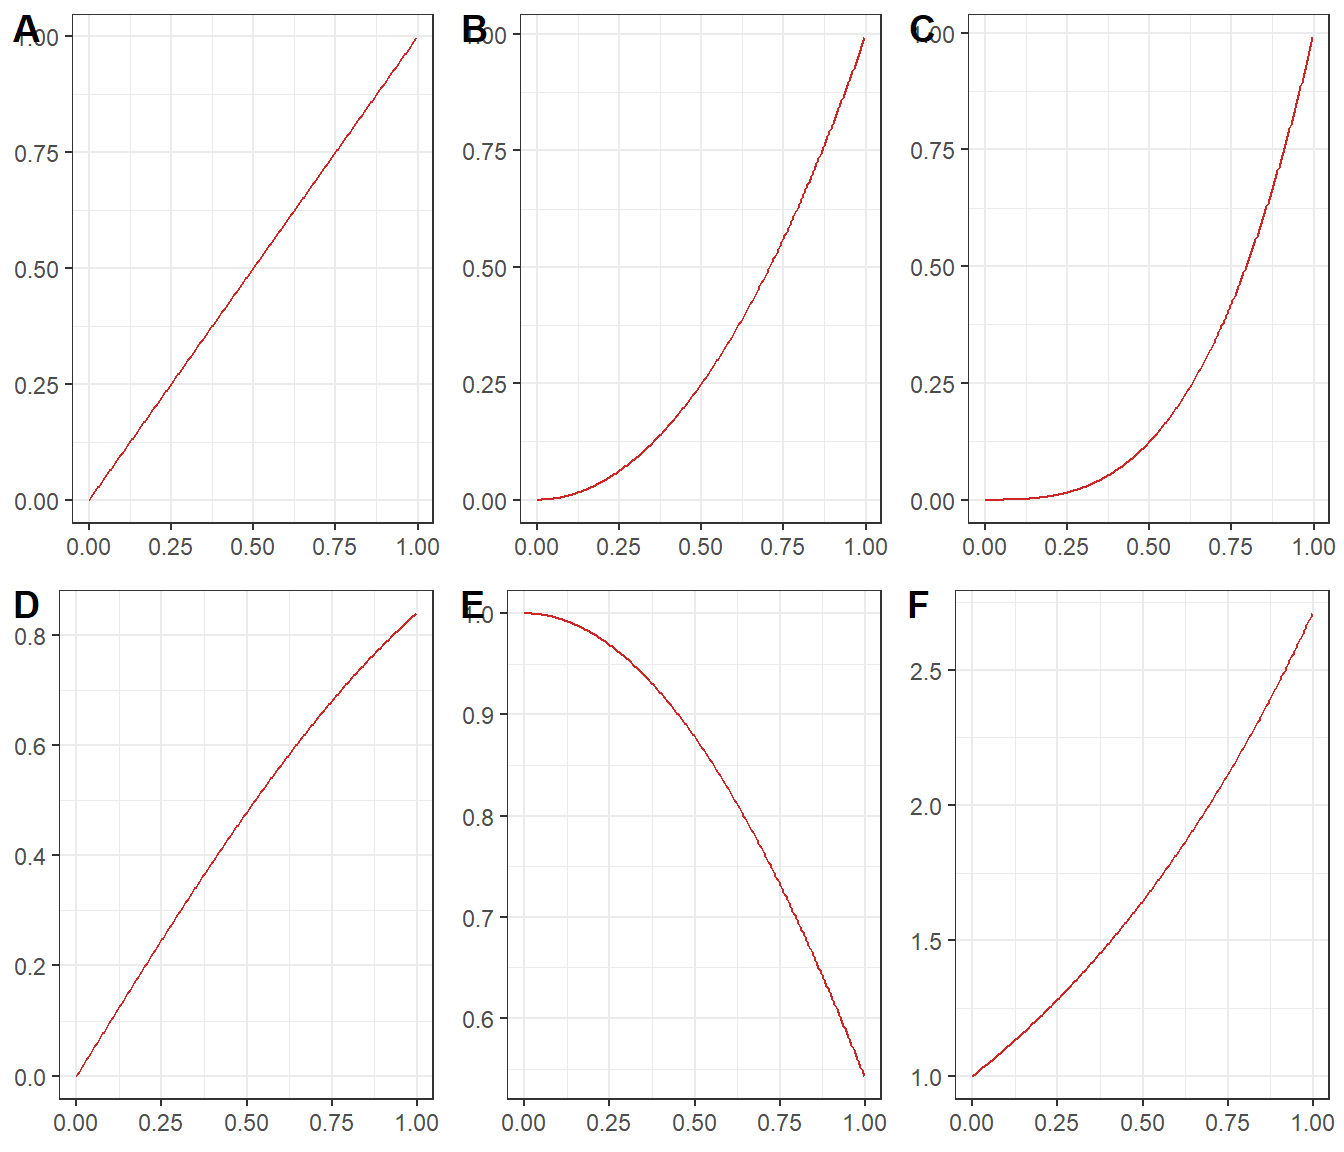
\includegraphics{thesis_files/figure-latex/Basicfunc-1} 

}

\caption{\label{fig:Basicplot}Plot of Basic functions analysed in this project}\label{fig:Basicfunc}
\end{figure}
In the figure \ref{fig:Basicplot} \textbf{A} is the \emph{Linear} function, \textbf{B} is the \emph{Quadratic} function, \textbf{C} is the \emph{Cubic} function, \textbf{D} is \emph{sinusoidal} function, \textbf{E} is \emph{cosinusoidal} function and \textbf{F} is \emph{Exponential} function. In addition to these basic functions the generated grid will be used to generate signals such as linchirp, Doppler, heavisine and the Mishmash. Definition of these signals is not simple; therefore, the plot of these signals has been provided in figure \ref{fig:Signals}.

Back to our simulation, after generating the grid from \(X \sim \text{unif}(0,1)\) the same procedure will be carried out for the data generated from a left skewed mixture of \(\text{beta}(2,1)\) and \(\text{unif}(0,1)\). And for the right skewed mixture of \(\text{beta}(1,2)\) and \(\text{unif}(0,1)\). These distributions have been generated using the regularized beta incomplete beta function from the \texttt{zipFR} package(Evert \& Baroni, 2007). The density plot of these distribution has been provided below:
\begin{figure}[htb!]

{\centering 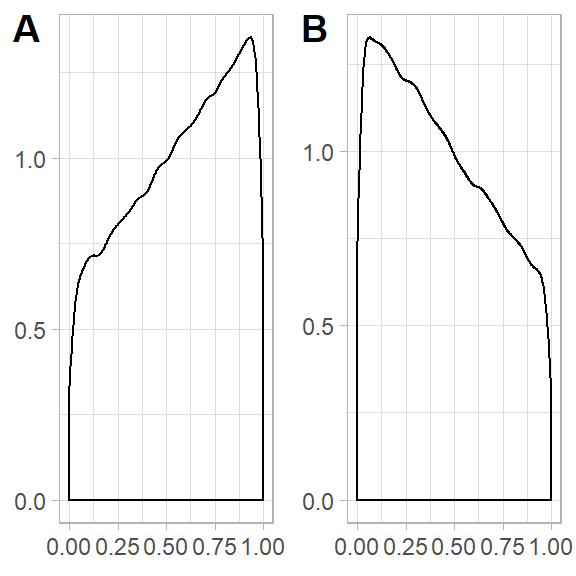
\includegraphics{thesis_files/figure-latex/skewed-1} 

}

\caption{\label{fig:skewed} Density plot of Left and Right skewed distrtibution used for generating grid}\label{fig:skewed}
\end{figure}
We have chosen these distribtions to make sure the generated grid point do start close to zero in a left-skewed case and do finish near one in the rightskewed case. In other words we wanted to have a grid which contain point from the entire \((0,1)\) interval and this is important because the true value \(f\) that we want to compare our estimates \(\hat f\) which is constructed from the previously mentioned functions and the equally spaced grid which starts from zero and goes all the way through one. It is important to try both left and right skewed grids and the reason for this is the non symmetric shape of signals. For instance, Doppler signals are more dense in the left hand side close to zero, so if the sample contains a small number of point on the right hand side it is not hard to see why some estimators will struggle to came up with a good estimate.

The signals in this project have been generate using the \texttt{make.signal2} in the \texttt{CNLTreg} (Nunes \& Knight, 2018) package in \textbf{R} which is a modified version of \texttt{make.signal} in \textbf{S-plus} and has the ability to generate signals on an specified grid. In addition, the plot in this project has been created using the \texttt{ggplot2} package (Wickham, 2016) and the \texttt{cowplot}(Wilke, 2019) has used to put the \texttt{ggplot} generated plots into a panel.
\begin{figure}[htb!]

{\centering 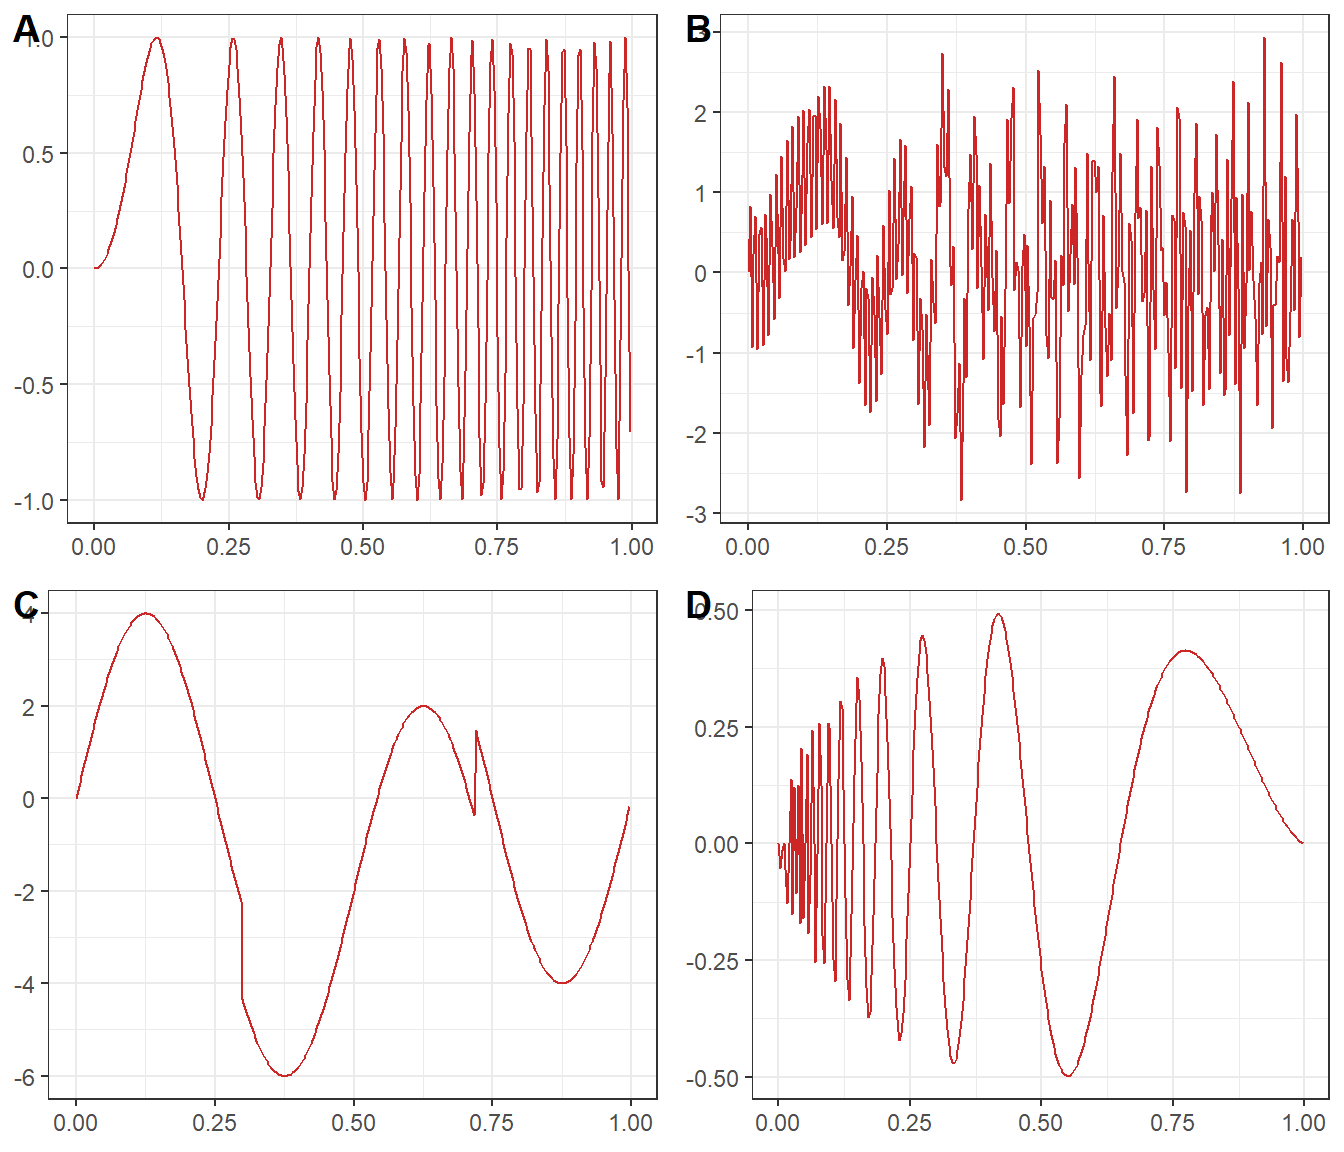
\includegraphics{thesis_files/figure-latex/Signals-1} 

}

\caption{\label{fig:Signals}Plot of signals analysed in this project}\label{fig:Signals}
\end{figure}
In figure \ref{fig:Signals} \textbf{A} is \texttt{Lincharp}, \textbf{B} is \texttt{Mishmash}, \textbf{C} is \texttt{Heavisine} and \textbf{D} is \texttt{Doppler}. Moreover, noise will be generated from a normal distribution with zero mean and a variance signal-to-noise ratio and will be added to the data. We will change the signal-to-noise ratio to observe the behavior of the estimators see \eqref{eq:noise}. The estimated values from the estimators will be recorded.

In this project four different estimators have been used to estimate the regression function. First, for \emph{first generation wavelet} the functions from \texttt{wavethresh} package. First we use the function \texttt{wd} which performs the wavelet discrete transform and then use \texttt{threshold} function drop the coefficent below the threshold and then we use function \texttt{wr} to perform the reverse wavelet trtansform. For these functions the parameters where kept as default. Second, for the \emph{second generation wavelet} the regression function from the \texttt{CNLTreg} package (Nunes \& Knight, 2018) has been used. This function gets takes the signal and grid value as argument returns the estimates. Parameter P in this
function is the number of times that the algorithm gets applied to the data then it
averages obtained estimates to obtain the final estimates. Moreover, selecting a P larger
than 2 is computationally intensive and according to our tests, in our does not
significantly improve the MSE, thus, we use P=2. Third, for \emph{kernel smoothing regression} \texttt{np} package (Hayfield \& Racine, 2008) has been used, this package contains all kind of nonparametric methods. The regression type for the \texttt{np} is chosen to be local constant and the bandwidth selection has been done by Kullback-leibler cross-validation(Hurvich, Simonoff, \& Tsai, 1998). Fourth, for \emph{spline} the \texttt{mgcv} package was used (Wood, 2003). This package has different functions built in to it including spline smoothing and generalized additive models. In this project to choose the optimal number of knots for penalized B-splines we have used the function gam.check which is provided in the package. The optimal K was 60 for all the signals. This is because the number of knots should be large enough to avoid underfitting. However, if the number of knots is more than enough it would avoid overfitting by penalizing term in equation \eqref{eq:RSS}.

\hypertarget{calculating-mse}{%
\section{Calculating MSE}\label{calculating-mse}}

Our purpose is to estimate the estimate \(f\) in equation below:
\begin{equation}
Y_{ij}=f(t_j)+\epsilon_{ij},\quad \epsilon\sim N(0,\sigma^2)
\label{eq:model}
\end{equation}
In \eqref{eq:model} we know that \(f(t)\) which is the true value of the function of interest. We obtain it by pluging an equally space grid with desirable amount of time points in the function. Furthermore, \(\sigma\) is calibrated by the following equation with respect to signal-to-noise-ratio \(r\):
\begin{equation}
\sigma^2=\frac{Var(f(t_i))}{r},\quad i=1,\dots,M
\label{eq:noise}
\end{equation}
Where \(t_i\) is a fixed grid of lenght \(M\), therefore \(f(t_i)\) is a vector of lenght \(M\) and we calculate the variance of it. In each iteration we calculate the estimate for each time point and record it. Therefore, after N iterations we have \(N\) estimate of length \(M\) for the signal of interest.
We have to note that for the estimators that take the unequal-spaced grid as an argument we have to interpolate the estimated value to a equal-space grid. This will allow us to compare different estimators by calculating the MSE. Now we will discus how to calculate MSE. The below formula will be used to calculate the MSE:
\[
\begin{aligned}
MSE=\mathbb{E}(\hat f,f)(t)&=\mathbb{E}(\hat f(t)-f(t))^2\\
&=\mathbb{E}[\hat f(t)-\mathbb{E}(\hat f(t))]+\mathbb{E}[\hat f(t))-f(t)]^2\\
&=\mathbb{E}[\hat f(t)-\mathbb{E}(\hat f(t))]^2+\mathbb{E}[Bias(\hat f(t),f(t))]^2\\
&=Var(\hat f(t))+Bias^2(\hat f(t),f(t))\\
\end{aligned}
\]
In the above formula \(f(t)\) is the true value of the function or signal \(f\) at point \(t\) which we wish to estimate. To obtain true value first we generate a equally space grid which is effectively a sequence of numbers with constant increment. Then we plug it in to our function and now we have the true values for each time \(t\). On the other hand, \(\hat f(t)\) is a the estimate that we get from our estimator. Using the same values we also use the following formula to calculate the Mean absolute error:
\[MAE=\mathbb{E}(|\hat f(t)- f(t)|)\].
We will use MAE because it is considered to be an alternative for MSE(Friedman, Hastie, \& Tibshirani, 2001).
As mentioned above after recording the estimates with length of M since the grid is of length \(M\) therefore the estimates would have the same length and associated interpolated values would have the same length too. Since we are repeated the procedure for N time we will end up with a dataset of interpolated estimated values which is a \(M\times N\) matrix. Although we mentioned interpolation is not good practice, we do it only for purpose of calculating the \emph{MSE} and \emph{MAE}. To calculate the bias of the estimates at point \(t\) we will take the average of the each row of the data set and subtract it from the true value of the regression function on that point. We calculate the variance of estimator at each point by simply calculating variance of each row of the data. Then we can calculate \emph{MSE} by the this formula \(MSE=Bias^2+Var\). Then we can calculate \(MSIE\) by calculating the mean of \(MSE\) of all points.

\hypertarget{results}{%
\chapter{Results}\label{results}}

\hypertarget{visual-pattern}{%
\section{Visual Pattern}\label{visual-pattern}}

In this chapter we will illustrate the result of the simulations. First we will start by showing some plots of different scenarios which in the estimations will be tested. The following graphs shows the scenario which the data of length 256 has been generated from a uniform distribution to make random grid is effectively non equally spaced and the curve \(f(x)=3x^3+4x^2\) is the function we want to estimate and the noise has been added to a signal-to-noise-ratio of 5. This curve has been chosen simply for demonstration purposes and we are primarily interested in estimating the function listed previously. Since this is a smooth function and the noise has been generated from a uniform distribution we expect that all the estimators could handle it well.
\begin{figure}[htb!]

{\centering 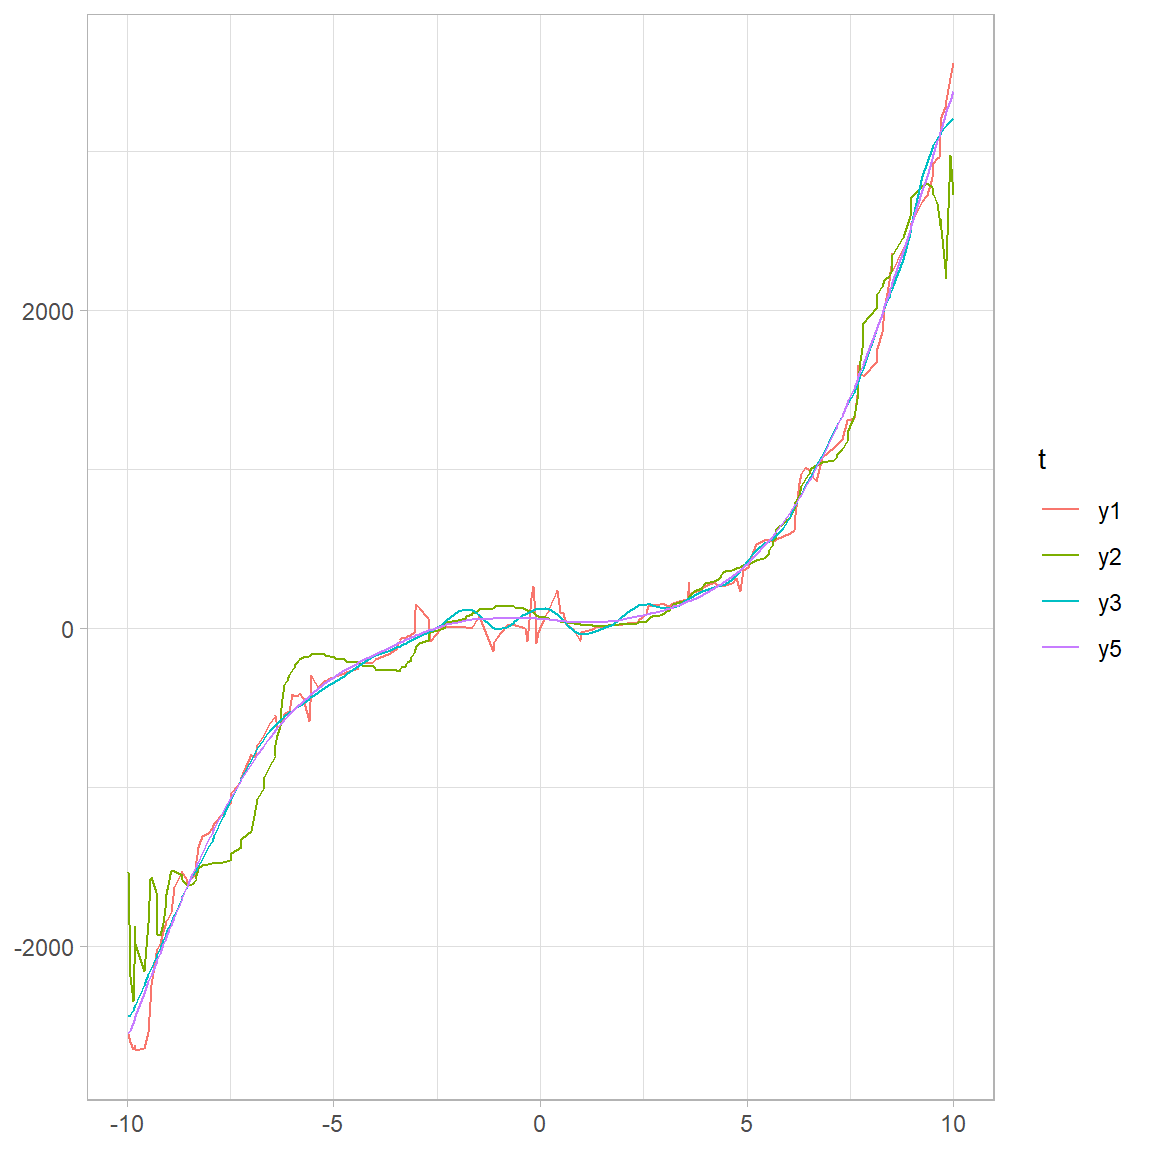
\includegraphics{thesis_files/figure-latex/basicunif-1} 

}

\caption{\label{fig:basicunif} Estimate of the the curve $f(x)=3x^3+4x^2$}\label{fig:basicunif1}
\end{figure}
\begin{figure}[htb!]

{\centering 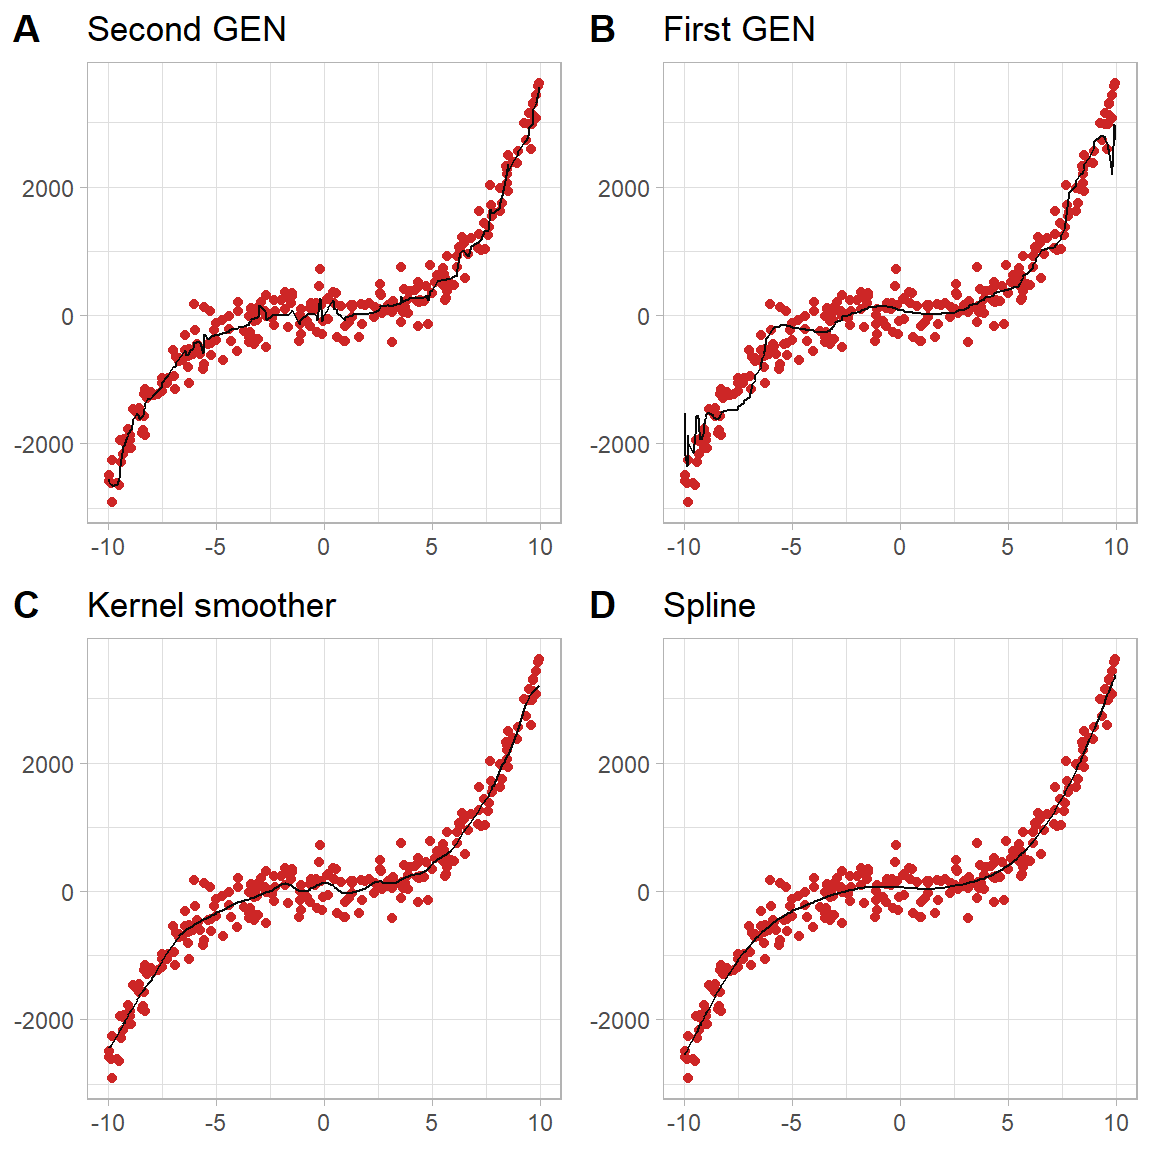
\includegraphics{thesis_files/figure-latex/basicunif-2} 

}

\caption{\label{fig:basicunif} Estimate of the the curve $f(x)=3x^3+4x^2$}\label{fig:basicunif2}
\end{figure}
As expected, figure \ref{fig:basicunif} show a good fit because there is not that much of variation in the data. Since the spline is less flexible than the other methods there is less variation in the spline estimated curve but obvious more biased and it is smoother.
In the next graph we will move on to a more challenging curve to estimate. Just like the previous example the data has been sampled from uniform distribution with length 256 and the ratio for noise is the same. The curve that we are keen to estimate is the Doppler signal. We showed this signal in the previous section and it has the property of this has a considerable amount of variation close to zero and as we move away from zero the variation decreases. This property will make the estimation hard for the less flexible estimator. Moreover, non equally spaced nature in the data should cause the first generation Wavelet to struggle.
\begin{figure}[htb!]

{\centering 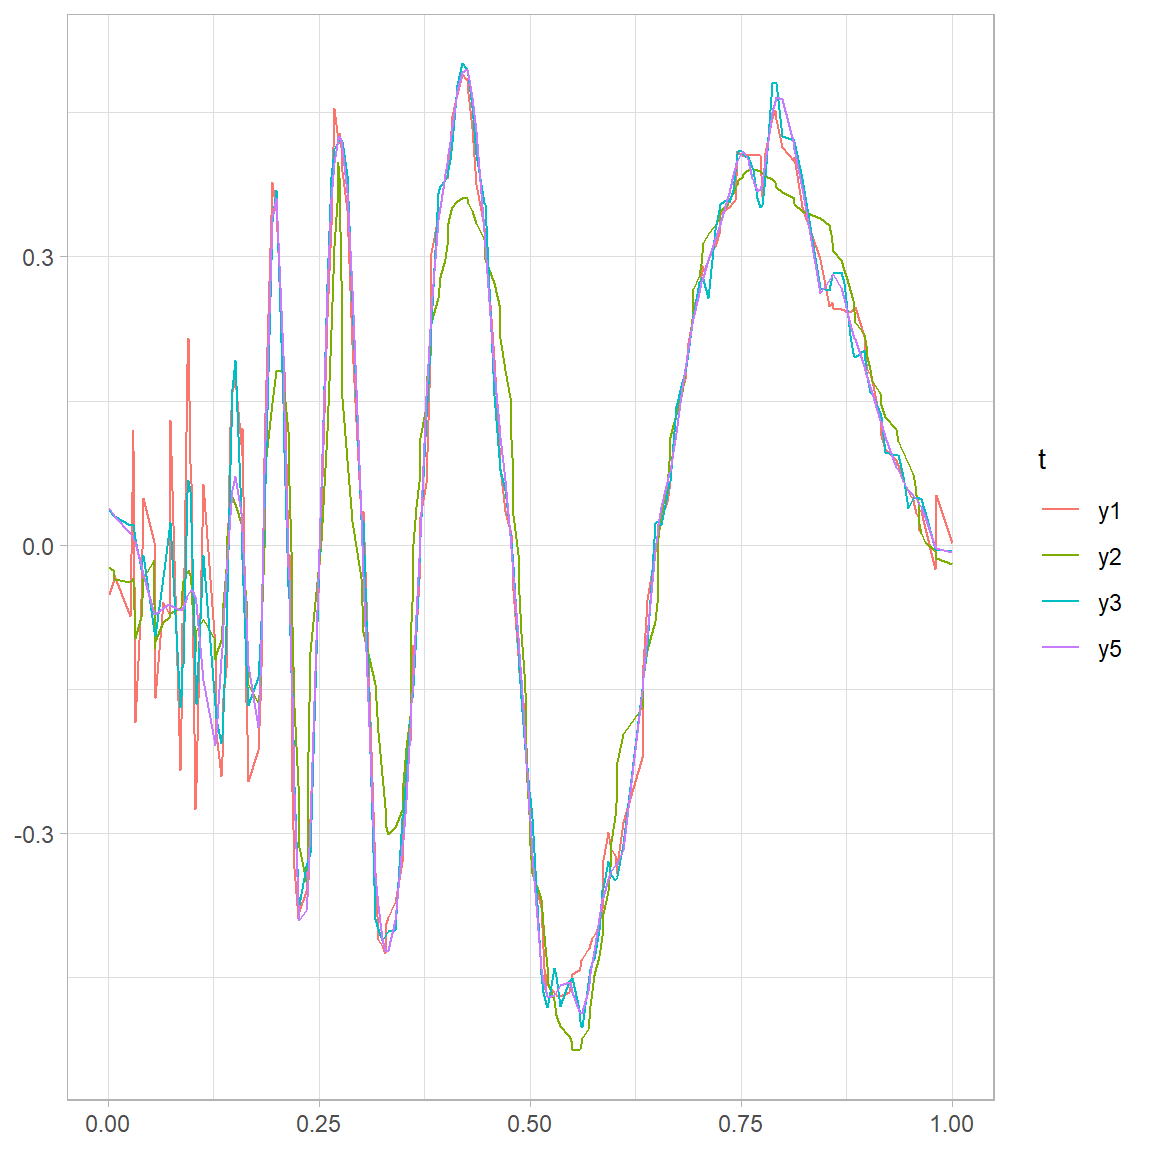
\includegraphics{thesis_files/figure-latex/unigridplot-1} 

}

\caption{\label{fig:unigridplot} Estimates of Doppler signal on a uniforn grid}\label{fig:unigridplot1}
\end{figure}
\begin{figure}[htb!]

{\centering 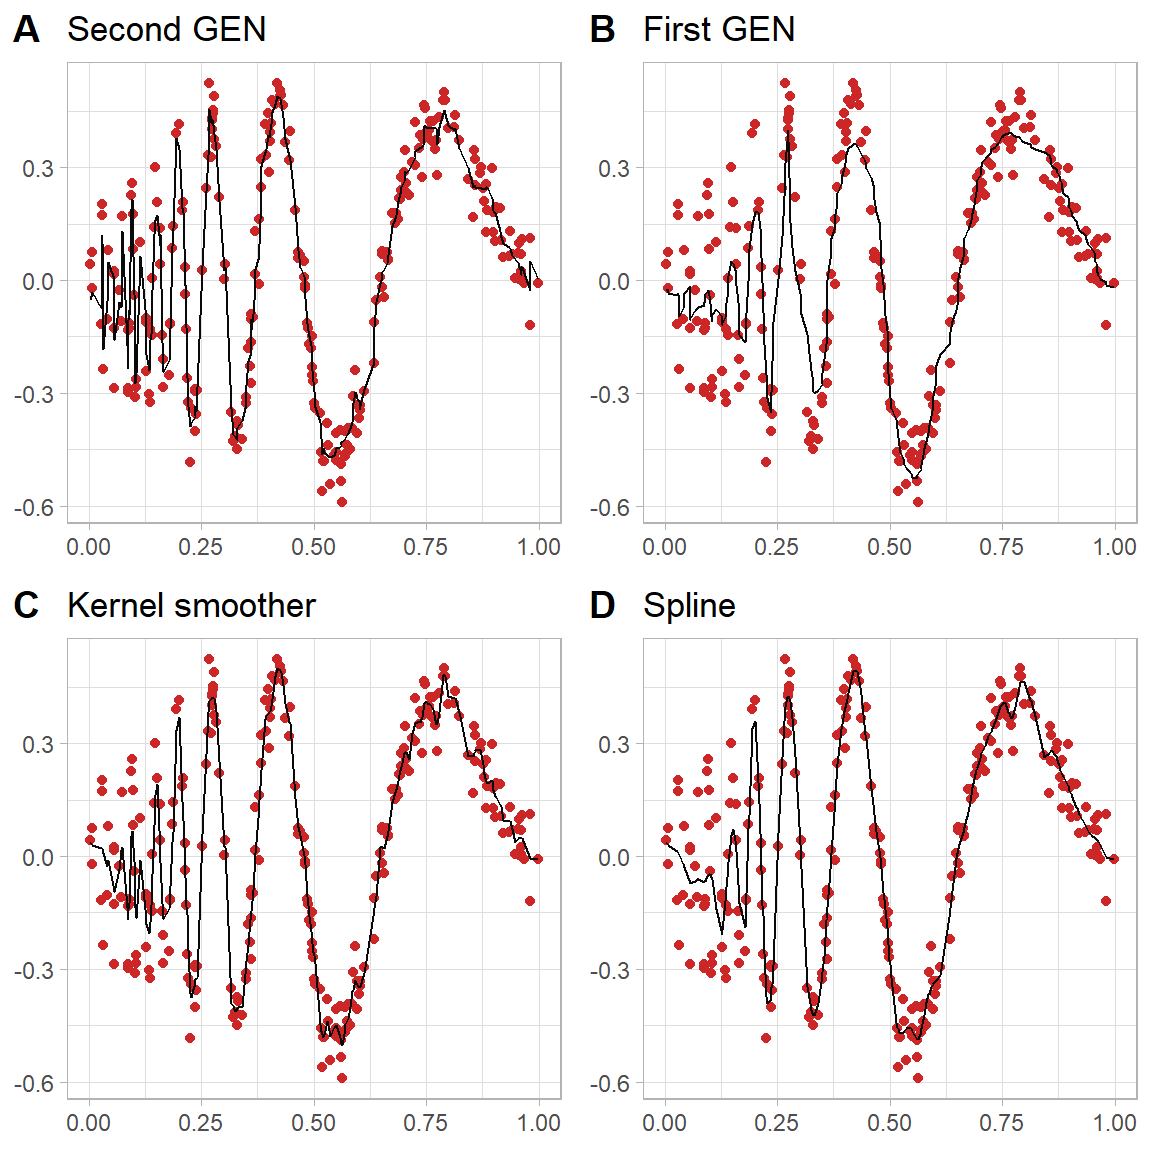
\includegraphics{thesis_files/figure-latex/unigridplot-2} 

}

\caption{\label{fig:unigridplot} Estimates of Doppler signal on a uniforn grid}\label{fig:unigridplot2}
\end{figure}
According to the graphs \ref{fig:unigridplot} \emph{spline} estimator (D) could not capture the variation \(f\) when x is close to zero and it has avoided the peaks and it is biased. \emph{First generation Wavelet} estimator(B) has explained some variation close to zero and it is similar to spline in the essence that struggles to capture the peaks in the data.
In the next example the signal remains the same but the data will be generated from rigght-skewed to make it right-skewed. For this particular curve because the first half has more variation, having more data there will make it rather easier to estimate.
\begin{figure}[htb!]

{\centering 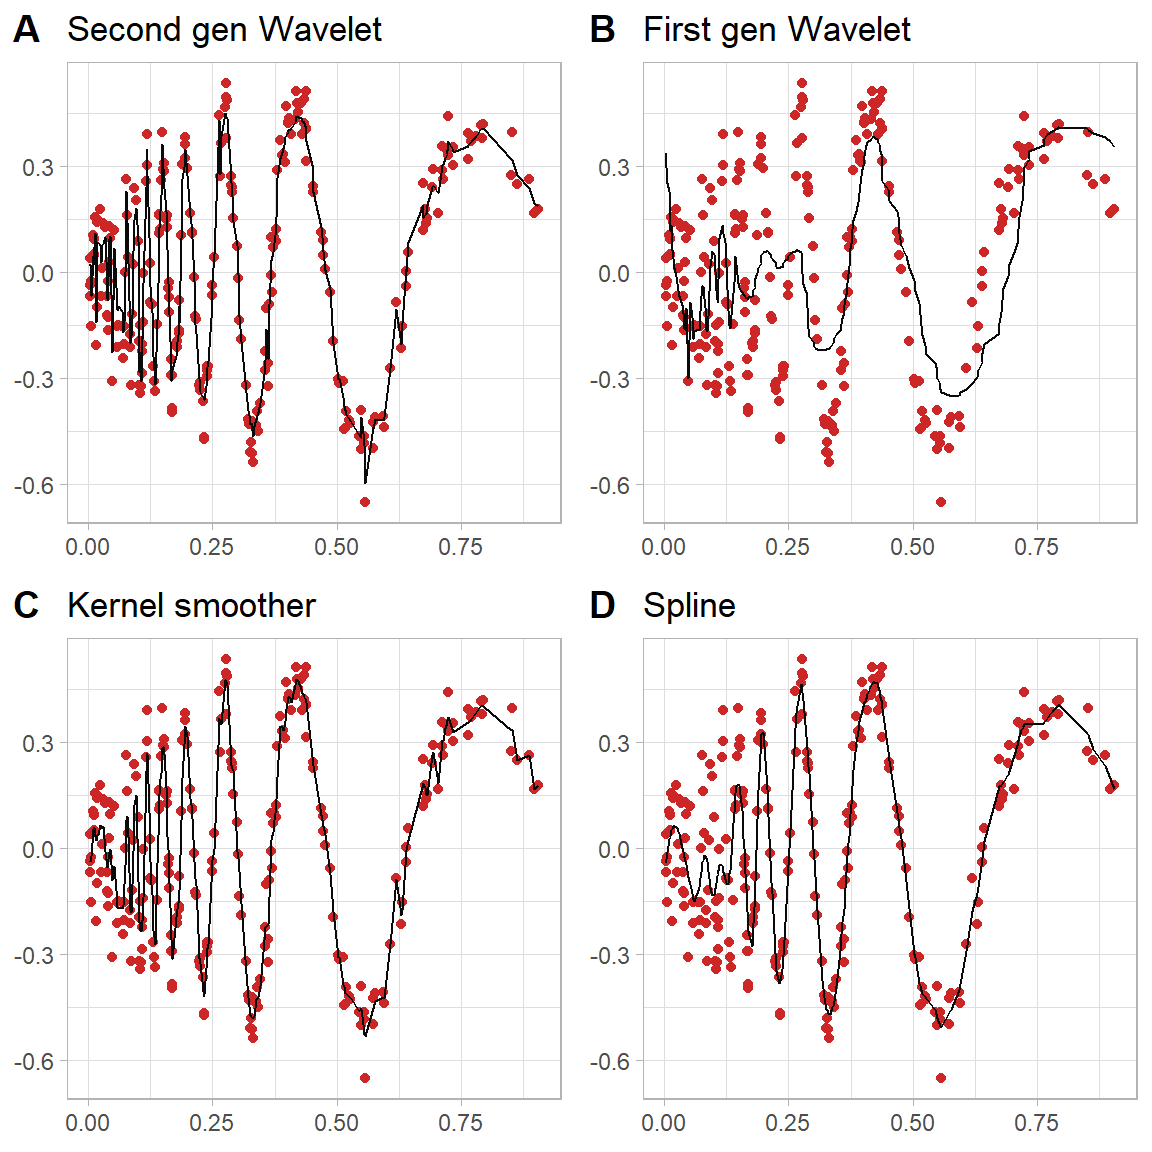
\includegraphics{thesis_files/figure-latex/rightgridplot-1} 

}

\caption{ \label{fig:rightgridplot} Estimate of Doppler signal on a right-skewewd grid}\label{fig:rightgridplot}
\end{figure}
As expected the same trend has happened in the graph \ref{fig:rightgridplot} \emph{second generation Wavelet}(A) and \emph{Kernel smoother}(C) estimators have done a good job but the other two are struggling. In next scenario we are going to generate the data from a left-skewed distribution and this means the first will have less data points close to zero. Therefore, we expect less flexible estimators to estimate the neighborhood around the zero.
\begin{figure}[htb!]

{\centering 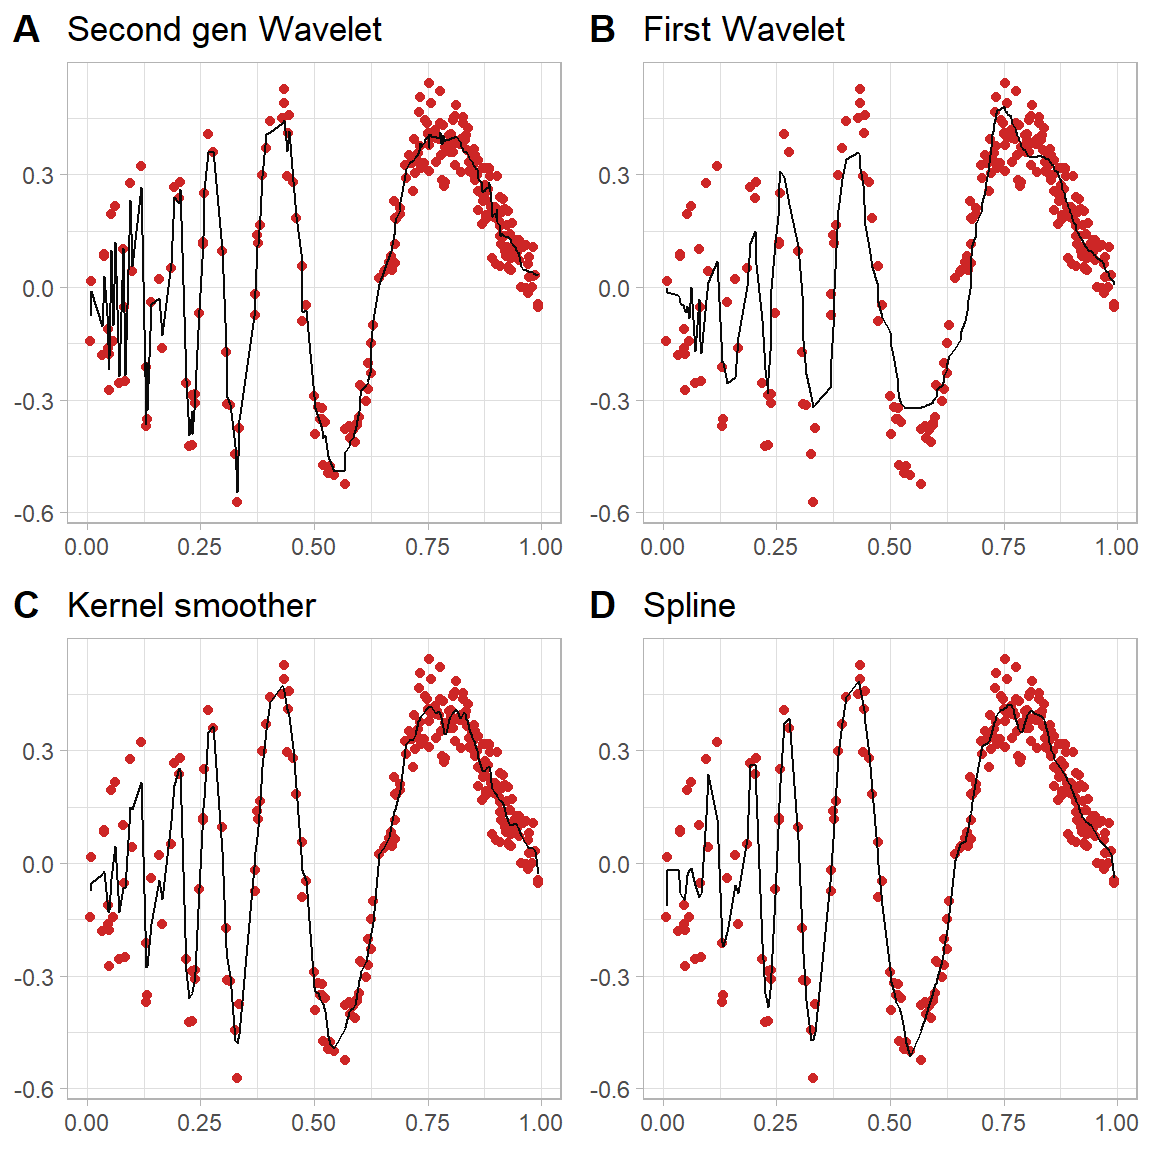
\includegraphics{thesis_files/figure-latex/leftgridplot-1} 

}

\caption{\label{fig:leftgridplot}Estimates of a Doppler signal left-skewed grid}\label{fig:leftgridplot}
\end{figure}
The figure \ref{fig:leftgridplot} shows almost all estimators are biased near biased close to zero. The first generation has done worse and still far from being perfect it has avoided most of the peaks. The other three etimators have done a good job at capturing most of the variation and the peaks in the data. This result indicated as we mentioned before the second generation estimators is most of the time as good as other commonly used nonparametric estimators. However, we wish test this to simulated the data multiple time and calculated \emph{MSE} and \emph{MAE} to investigate this in a more precise way.

\hypertarget{basic-functions}{%
\section{Basic functions}\label{basic-functions}}

In this part we will present the results of simulation on some familiar functions including identity, quadratic, cubic, sine, cosine and exp. For this simulation data has been generated from \(\text{unif}(0,1)\) we will run the simulation for 50 time and the grid length will be 256. The signal-to-noise ratio has been kept 5 for this simulation. The results has been given below:
\begin{longtable}[]{@{}ccccc@{}}
\caption{\label{tbl:msebasicunif5}MSE of estimates on signal on uniform grid with signal-to-noise-ratio 5 (continued below)}\tabularnewline
\toprule
estimators & Linear & Quad & Cubic & Sin\tabularnewline
\midrule
\endfirsthead
\toprule
estimators & Linear & Quad & Cubic & Sin\tabularnewline
\midrule
\endhead
First GEN & 1.148 & 1.078 & 0.944 & 0.8078\tabularnewline
Second GEN & \textbf{0.8524} & 0.9862 & \textbf{0.7771} & 0.6987\tabularnewline
Kernel smoother & 0.8526 & 0.9864 & 0.7774 & 0.6988\tabularnewline
Spline & 0.8524 & \textbf{0.9862} & 0.7771 & \textbf{0.6987}\tabularnewline
\bottomrule
\end{longtable}
\begin{longtable}[]{@{}cc@{}}
\toprule
Cos & Exp\tabularnewline
\midrule
\endhead
0.2671 & 3.323\tabularnewline
0.1898 & \textbf{2.411}\tabularnewline
0.1899 & 2.411\tabularnewline
\textbf{0.1898} & 2.411\tabularnewline
\bottomrule
\end{longtable}
\begin{longtable}[]{@{}ccccc@{}}
\caption{\label{tbl:maebasicunif5}MAE of estimates on signal on uniform grid with signal-to-noise-ratio 5 (continued below)}\tabularnewline
\toprule
estimators & Linear & Quad & Cubic & Sin\tabularnewline
\midrule
\endfirsthead
\toprule
estimators & Linear & Quad & Cubic & Sin\tabularnewline
\midrule
\endhead
First GEN & 13.67 & 13.15 & 12 & 11.76\tabularnewline
Second GEN & \textbf{11.86} & \textbf{12.64} & \textbf{10.46} & 10.84\tabularnewline
Kernel smoother & 11.86 & 12.64 & 10.47 & 10.84\tabularnewline
Spline & 11.86 & 12.64 & 10.46 & \textbf{10.84}\tabularnewline
\bottomrule
\end{longtable}
\begin{longtable}[]{@{}cc@{}}
\toprule
Cos & Exp\tabularnewline
\midrule
\endhead
6.597 & 23.13\tabularnewline
\textbf{5.671} & \textbf{20.43}\tabularnewline
5.671 & 20.43\tabularnewline
5.671 & 20.43\tabularnewline
\bottomrule
\end{longtable}
The results in \ref{tbl:msebasicunif5} and \ref{tbl:maebasicunif5} shows under different conditions the second generation wavelet and kernel smoother and the spline can each be the best estimator based on MSE and MAE, whereas the first generation wavelet has a worse performance. The tables show that this pattern consstently. We continue with another table which represent the results for simulation on the list of signals the parameters and the generated grid is the same as above.

\hypertarget{signals}{%
\section{Signals}\label{signals}}

\hypertarget{uniform-grid}{%
\subsection{Uniform grid}\label{uniform-grid}}
\begin{longtable}[]{@{}ccccc@{}}
\caption{\label{tbl:mseunif5} MSE of estimates on signal on uniform grid with signal-to-noise-ratio 5}\tabularnewline
\toprule
estimators & linchirp & mishmash & heavisine & doppler\tabularnewline
\midrule
\endfirsthead
\toprule
estimators & linchirp & mishmash & heavisine & doppler\tabularnewline
\midrule
\endhead
First GEN & 151.7 & 389.9 & 141.9 & 14.73\tabularnewline
Second GEN & \textbf{10.38} & 221.1 & \textbf{90.6} & \textbf{1.554}\tabularnewline
Kernel smoother & 13.9 & \textbf{220.4} & 90.79 & 1.782\tabularnewline
Spline & 18.59 & 288 & 94.53 & 2.654\tabularnewline
\bottomrule
\end{longtable}
\begin{longtable}[]{@{}ccccc@{}}
\caption{\label{tbl:maeunif5}MAE of estimates on signal on uniform grid with signal-to-noise-ratio 5}\tabularnewline
\toprule
estimators & linchirp & mishmash & heavisine & doppler\tabularnewline
\midrule
\endfirsthead
\toprule
estimators & linchirp & mishmash & heavisine & doppler\tabularnewline
\midrule
\endhead
First GEN & 158.6 & 256.6 & 156.8 & 45.31\tabularnewline
Second GEN & \textbf{34.56} & 184.5 & \textbf{126.2} & \textbf{15.05}\tabularnewline
Kernel smoother & 39.44 & \textbf{179} & 126.3 & 15.93\tabularnewline
Spline & 46.96 & 219.8 & 128.2 & 18.09\tabularnewline
\bottomrule
\end{longtable}
The results in \ref{tbl:mseunif5} and \ref{tbl:maeunif5} show the first generation is not doing a performing well on the signal linchirp ,whereas the other three are relatively good. For the next signal \emph{mishmash} the patterns gets repeated in both MSE and MAE the seconds generation very close to Kernel smoother. For the \emph{heavisine} the same pattern gets repeated. At last, all the estimators seems to have better performance in performance to the first generation for the \emph{doppler} signal both in MSE and MAE
Now we will decrease the signal to noise ratio to 3 for the next simulation but all the parameter will be kept constant.
\begin{longtable}[]{@{}ccccc@{}}
\caption{\label{tbl:mseunif3} MSE of estimates on signal on uniform grid with signal-to-noise-ratio 3}\tabularnewline
\toprule
estimators & linchirp & mishmash & heavisine & doppler\tabularnewline
\midrule
\endfirsthead
\toprule
estimators & linchirp & mishmash & heavisine & doppler\tabularnewline
\midrule
\endhead
First GEN & 133.3 & 399.9 & 735.2 & 17.84\tabularnewline
Second GEN & \textbf{16.88} & \textbf{238.4} & 277.7 & \textbf{2.77}\tabularnewline
Kernel smoother & 18.63 & 306.5 & \textbf{277.6} & 2.956\tabularnewline
Spline & 120.8 & 392.5 & 291.4 & 9.612\tabularnewline
\bottomrule
\end{longtable}
\begin{longtable}[]{@{}ccccc@{}}
\caption{\label{tbl:maeunif3}MAE of estimates on signal on uniform grid with signal-to-noise-ratio 3}\tabularnewline
\toprule
estimators & linchirp & mishmash & heavisine & doppler\tabularnewline
\midrule
\endfirsthead
\toprule
estimators & linchirp & mishmash & heavisine & doppler\tabularnewline
\midrule
\endhead
First GEN & 160 & 258.6 & 346.1 & 47.19\tabularnewline
Second GEN & \textbf{48.06} & \textbf{188.8} & 212.6 & \textbf{19.72}\tabularnewline
Kernel smoother & 50.5 & 223 & \textbf{212.6} & 20.29\tabularnewline
Spline & 147.8 & 257 & 218.1 & 37.08\tabularnewline
\bottomrule
\end{longtable}
Tables \ref{tbl:mseunif3} and \ref{tbl:maeunif3} show that decreasing the signal-noise-ratio to three which effetively icraeses the variation has triggered an increasing pattern in both MSE and MAE. However, the relation between the performance of the estimators has remained the same. The second generation seems to be the estimator execpt for the heavisine in which Kernel smoother seems to be better. Now we will increase the signal to ratio to 6 but all the other parameter will be kept constant.
\begin{longtable}[]{@{}ccccc@{}}
\caption{\label{tbl:mseunif6}MSE of estimates on signal on uniform grid with signal-to-noise-ratio 6}\tabularnewline
\toprule
estimators & linchirp & mishmash & heavisine & doppler\tabularnewline
\midrule
\endfirsthead
\toprule
estimators & linchirp & mishmash & heavisine & doppler\tabularnewline
\midrule
\endhead
First GEN & 104.4 & 387 & 231.7 & 8.585\tabularnewline
Second GEN & \textbf{5.247} & \textbf{208.5} & 53.46 & \textbf{1.054}\tabularnewline
Kernel smoother & 6.996 & 272.3 & \textbf{53.38} & 1.202\tabularnewline
Spline & 115.7 & 361.9 & 69.62 & 7.877\tabularnewline
\bottomrule
\end{longtable}
\begin{longtable}[]{@{}ccccc@{}}
\caption{\label{tbl:maeunif6}MAE of estimates on signal on uniform grid with signal-to-noise-ratio 6}\tabularnewline
\toprule
estimators & linchirp & mishmash & heavisine & doppler\tabularnewline
\midrule
\endfirsthead
\toprule
estimators & linchirp & mishmash & heavisine & doppler\tabularnewline
\midrule
\endhead
First GEN & 135.7 & 256.2 & 176.5 & 33.44\tabularnewline
Second GEN & \textbf{26.3} & \textbf{180.4} & 90.78 & \textbf{11.4}\tabularnewline
Kernel smoother & 29.89 & 214.4 & \textbf{90.73} & 11.99\tabularnewline
Spline & 144 & 250 & 103.8 & 31.67\tabularnewline
\bottomrule
\end{longtable}
The above results in table \ref{tbl:mseunif6} and \ref{tbl:maeunif6} are every similar to the results of the noise ratio 5. Now we will move on with testing left-skewed grid in the next section.

\hypertarget{left-skewed-grid}{%
\subsection{Left skewed grid}\label{left-skewed-grid}}
\begin{longtable}[]{@{}ccccc@{}}
\caption{\label{tbl:msebetaleft4}MSE of estimates on signal on Left-skewed grid with signal-to-noise-ratio 4}\tabularnewline
\toprule
estimators & linchirp & mishmash & heavisine & doppler\tabularnewline
\midrule
\endfirsthead
\toprule
estimators & linchirp & mishmash & heavisine & doppler\tabularnewline
\midrule
\endhead
First GEN & 123.5 & 382.6 & 1376 & 33.87\tabularnewline
Second GEN & \textbf{7.568} & \textbf{209.2} & \textbf{169.2} & \textbf{1.887}\tabularnewline
Kernel smoother & 9.662 & 382.8 & 169.3 & 1.95\tabularnewline
Spline & 123.8 & 386.1 & 188.4 & 9.14\tabularnewline
\bottomrule
\end{longtable}
\begin{longtable}[]{@{}ccccc@{}}
\caption{\label{tbl:maebetaleft4}MAE of estimates on a Left-skewed grid with signal-to-noise-ratio 4}\tabularnewline
\toprule
estimators & linchirp & mishmash & heavisine & doppler\tabularnewline
\midrule
\endfirsthead
\toprule
estimators & linchirp & mishmash & heavisine & doppler\tabularnewline
\midrule
\endhead
First GEN & 154.3 & 256 & 458.8 & 70.04\tabularnewline
Second GEN & \textbf{32.77} & \textbf{184.7} & \textbf{155.1} & \textbf{15.67}\tabularnewline
Kernel smoother & 37.05 & 258.4 & 155.2 & 15.89\tabularnewline
Spline & 155.5 & 259.8 & 165.2 & 34.96\tabularnewline
\bottomrule
\end{longtable}
Based on results in table \ref{tbl:msebetaleft4} and \ref{tbl:maebetaleft4} on both MSE and MAE second generation wavelet estimator performs better than the first generation wavelet estimator. In addition, it seems the left skewed nature of the grid had a profound impact on accuracy of the other estimators too. Thereby, second generation wavelet estimator has beat all of them this time. Although, the kernel smoother is a very close in most of case for example the MAEs for example for heavisine. In the next part we will increase the signal-to-noise ratio to 5 to observe the changes.
\begin{longtable}[]{@{}ccccc@{}}
\caption{\label{tbl:msebetaleft5}MSE of estimates on a Left-skewed grid with signal-to-noise-ratio 5}\tabularnewline
\toprule
estimators & linchirp & mishmash & heavisine & doppler\tabularnewline
\midrule
\endfirsthead
\toprule
estimators & linchirp & mishmash & heavisine & doppler\tabularnewline
\midrule
\endhead
First GEN & 144.9 & 383.2 & 2168 & 34.18\tabularnewline
Second GEN & \textbf{5.093} & \textbf{205.5} & \textbf{89.83} & \textbf{1.933}\tabularnewline
Kernel smoother & 7.124 & 210.6 & 89.83 & 1.969\tabularnewline
Spline & 113.1 & 374.1 & 106 & 8.357\tabularnewline
\bottomrule
\end{longtable}
\begin{longtable}[]{@{}ccccc@{}}
\caption{\label{tbl:maebetaleft5}MAE of estimates on a Left-skewed grid with signal-to-noise-ratio 5}\tabularnewline
\toprule
estimators & linchirp & mishmash & heavisine & doppler\tabularnewline
\midrule
\endfirsthead
\toprule
estimators & linchirp & mishmash & heavisine & doppler\tabularnewline
\midrule
\endhead
First GEN & 164.6 & 257.4 & 572.1 & 69.55\tabularnewline
Second GEN & \textbf{28.58} & 180 & 120 & \textbf{15.57}\tabularnewline
Kernel smoother & 33.16 & \textbf{176.2} & \textbf{120} & 16.16\tabularnewline
Spline & 144.4 & 254.2 & 129.8 & 33.34\tabularnewline
\bottomrule
\end{longtable}
Increasing the signal to noise ratio from 4 to 5 has increased the MSEs and MAEs for the heavisine of first generation wavelet method sunbstantially according to tables \ref{tbl:msebetaleft5} and \ref{tbl:maebetaleft5}. In contrast, both MSE and MAE for the other signals have not change significantly. Overall relations between different estimators is similar to the previous simulation except in the MAE table Kernel smoother is slighty better than second generation for mishmash and heavisine. Now will will increase the signal-to noise ratio to 6.
\begin{longtable}[]{@{}ccccc@{}}
\caption{\label{tbl:msebetaleft6}MSE of estimates on a Left-skewed grid with signal-to-noise-ratio 6}\tabularnewline
\toprule
estimators & linchirp & mishmash & heavisine & doppler\tabularnewline
\midrule
\endfirsthead
\toprule
estimators & linchirp & mishmash & heavisine & doppler\tabularnewline
\midrule
\endhead
First GEN & 145.2 & 400 & 3330 & 34.53\tabularnewline
Second GEN & \textbf{6.858} & \textbf{185.8} & \textbf{65.09} & \textbf{1.099}\tabularnewline
Kernel smoother & 9.211 & 186.3 & 65.12 & 1.22\tabularnewline
Spline & 119.2 & 353.9 & 84.77 & 8.068\tabularnewline
\bottomrule
\end{longtable}
\begin{longtable}[]{@{}ccccc@{}}
\caption{\label{tbl:maebetaleft6}MAE of estimates on a Left-skewed grid with signal-to-noise-ratio 6}\tabularnewline
\toprule
estimators & linchirp & mishmash & heavisine & doppler\tabularnewline
\midrule
\endfirsthead
\toprule
estimators & linchirp & mishmash & heavisine & doppler\tabularnewline
\midrule
\endhead
First GEN & 163.1 & 259.2 & 735.4 & 73.14\tabularnewline
Second GEN & \textbf{31.41} & 171.4 & \textbf{103} & \textbf{12.32}\tabularnewline
Kernel smoother & 35.66 & \textbf{164.9} & 103 & 12.79\tabularnewline
Spline & 146.5 & 246.3 & 117.1 & 31.99\tabularnewline
\bottomrule
\end{longtable}
The results in \ref{tbl:msebetaleft6} and \ref{tbl:maebetaleft6} does not shows that much of difference from the the signal-to-noise ratio 5. The overall relations remain the same between estimators. Comparing the results to the uniformly generating grid MSE and MAE of first generation estimators has gone up for all the signals. However, they are very close to the previous part for other estimators.

\hypertarget{right-skewed-grid}{%
\subsection{Right skewed grid}\label{right-skewed-grid}}

In this part the grid is chosen to be right-skewed. The below table shows the simulation using signal to noise ratio 4 and the other parameter remain constant.
\begin{longtable}[]{@{}ccccc@{}}
\caption{\label{tbl:msebetaright4}MSE of estimates on a right-skewed grid with signal-to-noise-ratio 4}\tabularnewline
\toprule
estimators & linchirp & mishmash & heavisine & doppler\tabularnewline
\midrule
\endfirsthead
\toprule
estimators & linchirp & mishmash & heavisine & doppler\tabularnewline
\midrule
\endhead
First GEN & 136.5 & 447.1 & 3013 & 29.92\tabularnewline
Second GEN & \textbf{24.94} & \textbf{236} & \textbf{132.7} & \textbf{1.511}\tabularnewline
Kernel smoother & 26.59 & 251.2 & 132.9 & 1.634\tabularnewline
Spline & 124.9 & 396.9 & 154.1 & 8.329\tabularnewline
\bottomrule
\end{longtable}
\begin{longtable}[]{@{}ccccc@{}}
\caption{\label{tbl:maebetaright4}MAE of estimates on a right-skewed grid with signal-to-noise-ratio 4}\tabularnewline
\toprule
estimators & linchirp & mishmash & heavisine & doppler\tabularnewline
\midrule
\endfirsthead
\toprule
estimators & linchirp & mishmash & heavisine & doppler\tabularnewline
\midrule
\endhead
First GEN & 157.9 & 279.1 & 698.7 & 72.83\tabularnewline
Second GEN & \textbf{50.98} & 185.9 & \textbf{147.6} & \textbf{14.48}\tabularnewline
Kernel smoother & 52.51 & \textbf{183.7} & 147.8 & 15\tabularnewline
Spline & 151.2 & 260.1 & 157.6 & 33.41\tabularnewline
\bottomrule
\end{longtable}
In the table \ref{tbl:msebetaright4} the results for second generation and Kernel smoother are close. In contrast, the estimates for first generation is substantially larger. The same pattern can be observed in the \ref{tbl:maebetaright4}. Second generation wavelet method is the best except for the mishmash signal. In the following signal-to noise-ratio will be increase to 5.
\begin{longtable}[]{@{}ccccc@{}}
\caption{\label{tbl:msebetaright5}MSE of estimates on a right-skewed grid with signal-to-noise-ratio 5}\tabularnewline
\toprule
estimators & linchirp & mishmash & heavisine & doppler\tabularnewline
\midrule
\endfirsthead
\toprule
estimators & linchirp & mishmash & heavisine & doppler\tabularnewline
\midrule
\endhead
First GEN & 144.9 & 442.7 & 1390 & 47.83\tabularnewline
Second GEN & \textbf{7.783} & \textbf{224.6} & \textbf{118.1} & \textbf{1.324}\tabularnewline
Kernel smoother & 9.761 & 271.3 & 118.2 & 1.561\tabularnewline
Spline & 113.6 & 367.5 & 132.2 & 8.326\tabularnewline
\bottomrule
\end{longtable}
\begin{longtable}[]{@{}ccccc@{}}
\caption{\label{tbl:maebetaright5}MAE of estimates on a right-skewed grid with signal-to-noise-ratio 5}\tabularnewline
\toprule
estimators & linchirp & mishmash & heavisine & doppler\tabularnewline
\midrule
\endfirsthead
\toprule
estimators & linchirp & mishmash & heavisine & doppler\tabularnewline
\midrule
\endhead
First GEN & 158 & 268.1 & 475.3 & 89.54\tabularnewline
Second GEN & \textbf{28.57} & \textbf{184.6} & \textbf{113.7} & \textbf{12.58}\tabularnewline
Kernel smoother & 33.07 & 210.9 & 113.8 & 13.38\tabularnewline
Spline & 143.9 & 248.1 & 125.4 & 32\tabularnewline
\bottomrule
\end{longtable}
According to table \ref{tbl:msebetaright5} and \ref{tbl:maebetaright5} change in signal-to-noise-ratio does not change the estimates substantially; however, the estimates of the heavisine seems to decrease both in \ref{tbl:msebetaright5} and \ref{tbl:maebetaright5}. In the following able the signal-to-noise-ratio will be increased to 6.
\begin{longtable}[]{@{}ccccc@{}}
\caption{\label{tbl:msebetaright6}MSE of estimates on a right-skewed grid with signal-to-noise-ratio 6}\tabularnewline
\toprule
estimators & linchirp & mishmash & heavisine & doppler\tabularnewline
\midrule
\endfirsthead
\toprule
estimators & linchirp & mishmash & heavisine & doppler\tabularnewline
\midrule
\endhead
First GEN & 1.91 & 1.642 & 2.502 & 1.711\tabularnewline
Second GEN & \textbf{0.7898} & \textbf{0.5211} & \textbf{0.4299} & \textbf{0.4406}\tabularnewline
Kernel smoother & 0.7898 & 0.5216 & 0.4299 & 0.4407\tabularnewline
Spline & 0.7898 & 0.5211 & 0.4299 & 0.4406\tabularnewline
\bottomrule
\end{longtable}
\begin{longtable}[]{@{}ccccc@{}}
\caption{\label{tbl:maebetaright6}MAE of estimates on a right-skewed grid with signal-to-noise-ratio 6}\tabularnewline
\toprule
estimators & linchirp & mishmash & heavisine & doppler\tabularnewline
\midrule
\endfirsthead
\toprule
estimators & linchirp & mishmash & heavisine & doppler\tabularnewline
\midrule
\endhead
First GEN & 18.46 & 17.23 & 21.12 & 17.93\tabularnewline
Second GEN & 10.87 & \textbf{9.334} & 8.195 & 8.89\tabularnewline
Kernel smoother & 10.87 & 9.337 & 8.195 & \textbf{8.889}\tabularnewline
Spline & \textbf{10.87} & 9.334 & \textbf{8.195} & 8.89\tabularnewline
\bottomrule
\end{longtable}
For this analysis the results in both \ref{tbl:msebetaright6} and \ref{tbl:maebetaright6} are substantialy smaller than the previoous part, it seems that the signal-to-noise-ratio noticeably effect the estimates and pushed them down.

\hypertarget{conclusion}{%
\chapter{Conclusion}\label{conclusion}}

The simulations based on the basic functions did not show considerable difference between estimators. However, \emph{first generation wavelet} estimator had a higher MSE and MAE compared to other estimators in the basic function case. In case of signals with uniform grids and different signal-to-noise-ratio, second generation wavelet estimators had much smaller MSE and MAE than other estimator except for a small number of cases where nonparametric estimators has smaller MSE or MAE.

The results show that for the uniform grid cases and for all tested signal-to-noise-ratio, first generation wavelet had a much larger MSE and MAE compared to second generation method. Changing the grid to the left-skewed and right-skewed did not have any noticeable effect on the MSE and MAE of the second generation wavelet and kernel smoothing, but results an increase in the MSE and MAE of first generation and spline.

In conclusion, the results showed second generation wavelet estimator is a suitable and powerful tool for analyzing the datasets with irregular grid. In would be interesting to study this estimators in the case with more than one independent variable and comparing the results with other estimators and applying methods to time series data which are correlated.

\appendix

\hypertarget{appendix}{%
\chapter{Appendix}\label{appendix}}

The output below shows the codes and the function that has been used in this project:
\begin{Shaded}
\begin{Highlighting}[]
\KeywordTok{library}\NormalTok{(CNLTreg)}
\KeywordTok{library}\NormalTok{(tidyverse)}
\KeywordTok{library}\NormalTok{(cowplot)}
\NormalTok{n_t=}\DecValTok{300}
\NormalTok{t =}\StringTok{ }\KeywordTok{seq}\NormalTok{(}\DataTypeTok{from =} \DecValTok{0}\NormalTok{, }\DataTypeTok{to =} \DecValTok{1} \OperatorTok{-}\StringTok{ }\DecValTok{1}\OperatorTok{/}\NormalTok{n_t, }\DataTypeTok{by =} \DecValTok{1}\OperatorTok{/}\NormalTok{n_t)}
\NormalTok{signals<-}\KeywordTok{list}\NormalTok{(}\StringTok{"linchirp"}\NormalTok{,}\StringTok{"mishmash1"}\NormalTok{,}\StringTok{"heavisine"}\NormalTok{,}\StringTok{"doppler"}\NormalTok{)}
\KeywordTok{map}\NormalTok{(signals,}\ControlFlowTok{function}\NormalTok{(y) }\KeywordTok{make.signal2}\NormalTok{(y,}\DataTypeTok{x=}\NormalTok{t)) }\OperatorTok\StringTok{ }
\StringTok{  }\KeywordTok{map}\NormalTok{(}\ControlFlowTok{function}\NormalTok{(y) }\KeywordTok{ggplot}\NormalTok{(}\KeywordTok{as.data.frame}\NormalTok{(y),}\KeywordTok{aes}\NormalTok{(}\DataTypeTok{y=}\NormalTok{y,}\DataTypeTok{x=}\NormalTok{t))}\OperatorTok{+}
\StringTok{        }\KeywordTok{geom_line}\NormalTok{(}\DataTypeTok{color=}\StringTok{"firebrick3"}\NormalTok{)}\OperatorTok{+}\KeywordTok{theme_bw}\NormalTok{()}\OperatorTok{+}
\StringTok{        }\KeywordTok{theme}\NormalTok{(}\DataTypeTok{axis.title.x=}\KeywordTok{element_blank}\NormalTok{(),}
              \DataTypeTok{axis.title.y=}\KeywordTok{element_blank}\NormalTok{()))}\OperatorTok
\StringTok{  }\KeywordTok{plot_grid}\NormalTok{(}\DataTypeTok{plotlist =}\NormalTok{ .,}
            \DataTypeTok{labels =} \KeywordTok{c}\NormalTok{(}\StringTok{"A"}\NormalTok{,}\StringTok{"B"}\NormalTok{,}\StringTok{"C"}\NormalTok{,}\StringTok{"D"}\NormalTok{))}
\end{Highlighting}
\end{Shaded}
\begin{Shaded}
\begin{Highlighting}[]
\NormalTok{x1<-}\KeywordTok{sort}\NormalTok{(}\KeywordTok{runif}\NormalTok{(}\DecValTok{256}\NormalTok{,}\OperatorTok{-}\DecValTok{10}\NormalTok{,}\DecValTok{10}\NormalTok{))}
\NormalTok{y<-}\DecValTok{3}\OperatorTok{*}\NormalTok{x1}\OperatorTok{^}\DecValTok{3}\OperatorTok{+}\DecValTok{4}\OperatorTok{*}\NormalTok{x1}\OperatorTok{^}\DecValTok{2}
\NormalTok{noise<-}\KeywordTok{rnorm}\NormalTok{(}\DecValTok{256}\NormalTok{,}\DataTypeTok{mean=}\DecValTok{0}\NormalTok{,}\DataTypeTok{sd=}\KeywordTok{sqrt}\NormalTok{(}\KeywordTok{var}\NormalTok{(y))}\OperatorTok{/}\DecValTok{5}\NormalTok{)}
\NormalTok{y<-y}\OperatorTok{+}\NormalTok{noise }
\NormalTok{est1<-CNLTreg}\OperatorTok{::}\KeywordTok{cnlt.reg}\NormalTok{(x1,y,}\DataTypeTok{P=}\DecValTok{2}\NormalTok{,}
                        \DataTypeTok{LocalPred=}\NormalTok{AdaptPred,}\DataTypeTok{neighbours=}\DecValTok{1}\NormalTok{,}
                        \DataTypeTok{returnall=}\OtherTok{FALSE}\NormalTok{)}
\NormalTok{estwd <-}\StringTok{ }\NormalTok{wavethresh}\OperatorTok{::}\KeywordTok{wd}\NormalTok{(y)}
\NormalTok{estwr <-}\StringTok{ }\NormalTok{wavethresh}\OperatorTok{::}\StringTok{ }\KeywordTok{wr}\NormalTok{(wavethresh}\OperatorTok{::}\KeywordTok{threshold}\NormalTok{(estwd,}
                                               \DataTypeTok{by.level=}\OtherTok{TRUE}\NormalTok{,}
                                               \DataTypeTok{policy=}\StringTok{"universal"}\NormalTok{)) }

\NormalTok{npbwrh <-np}\OperatorTok{::}\StringTok{ }\KeywordTok{npregbw}\NormalTok{(y }\OperatorTok{~}\StringTok{ }\NormalTok{x1, }\DataTypeTok{regtype =} \StringTok{"lc"}\NormalTok{,}
                      \DataTypeTok{bwmethod =} \StringTok{"cv.aic"}\NormalTok{)}
\NormalTok{nprh1 <-}\StringTok{ }\NormalTok{np}\OperatorTok{::}\KeywordTok{npreg}\NormalTok{(npbwrh)}


\NormalTok{bk <-}\StringTok{ }\NormalTok{mgcv}\OperatorTok{::}\StringTok{ }\KeywordTok{gam}\NormalTok{(y}\OperatorTok{~}\StringTok{ }\KeywordTok{s}\NormalTok{(x1,}\DataTypeTok{bs=}\StringTok{"ps"}\NormalTok{,}\DataTypeTok{k=}\DecValTok{60}\NormalTok{),}\DataTypeTok{family=}\NormalTok{gaussian)}
\NormalTok{bk<-bk}\OperatorTok{$}\NormalTok{fitted.values}

\NormalTok{estfr<-}\KeywordTok{cbind.data.frame}\NormalTok{(x1,y,}
                        \DataTypeTok{y1=}\KeywordTok{t}\NormalTok{(est1),}
                        \DataTypeTok{y2=}\NormalTok{estwr,}
                        \DataTypeTok{y3=}\KeywordTok{fitted}\NormalTok{(nprh1),}
                        \DataTypeTok{y5=}\NormalTok{bk)}
\NormalTok{estfr1<-}\StringTok{ }\NormalTok{estfr }\OperatorTok\StringTok{ }\KeywordTok{gather}\NormalTok{(}\DataTypeTok{key=}\StringTok{"t"}\NormalTok{,}\DataTypeTok{value=}\StringTok{"para"}\NormalTok{,y1,y2,y3,y5)}



\NormalTok{estfr1 }\OperatorTok\StringTok{ }\KeywordTok{ggplot}\NormalTok{(}\KeywordTok{aes}\NormalTok{(}\DataTypeTok{x=}\NormalTok{x1,}\DataTypeTok{y=}\NormalTok{para,}\DataTypeTok{color=}\NormalTok{t,}\DataTypeTok{group=}\NormalTok{t))}\OperatorTok{+}\KeywordTok{geom_line}\NormalTok{()}\OperatorTok{+}\KeywordTok{theme_light}\NormalTok{()}\OperatorTok{+}\KeywordTok{theme}\NormalTok{(}\DataTypeTok{axis.title.x=}\KeywordTok{element_blank}\NormalTok{(),}\DataTypeTok{axis.title.y=}\KeywordTok{element_blank}\NormalTok{())}



\NormalTok{pr1<-}\KeywordTok{ggplot}\NormalTok{(estfr,}\KeywordTok{aes}\NormalTok{(}\DataTypeTok{x=}\NormalTok{ x1,}\DataTypeTok{y=}\NormalTok{ y))}\OperatorTok{+}
\StringTok{  }\KeywordTok{geom_point}\NormalTok{(}\DataTypeTok{color=}\StringTok{"firebrick3"}\NormalTok{)}\OperatorTok{+}
\StringTok{  }\KeywordTok{geom_line}\NormalTok{(}\KeywordTok{aes}\NormalTok{(}\DataTypeTok{x=}\NormalTok{x1,}\DataTypeTok{y=}\NormalTok{y1),}\DataTypeTok{color=}\StringTok{"gray4"}\NormalTok{)}\OperatorTok{+}
\StringTok{  }\KeywordTok{ggtitle}\NormalTok{(}\StringTok{"Second GEN"}\NormalTok{)}\OperatorTok{+}\KeywordTok{theme_light}\NormalTok{()}\OperatorTok{+}\StringTok{ }\KeywordTok{theme}\NormalTok{(}\DataTypeTok{axis.title.x=}\KeywordTok{element_blank}\NormalTok{(),}\DataTypeTok{axis.title.y=}\KeywordTok{element_blank}\NormalTok{())}


\NormalTok{pr2<-}\KeywordTok{ggplot}\NormalTok{(estfr,}\KeywordTok{aes}\NormalTok{(}\DataTypeTok{x=}\NormalTok{ x1,}\DataTypeTok{y=}\NormalTok{y))}\OperatorTok{+}
\StringTok{  }\KeywordTok{geom_point}\NormalTok{(}\DataTypeTok{color=}\StringTok{"firebrick3"}\NormalTok{)}\OperatorTok{+}
\StringTok{  }\KeywordTok{geom_line}\NormalTok{(}\KeywordTok{aes}\NormalTok{(}\DataTypeTok{x=}\NormalTok{x1,}\DataTypeTok{y=}\NormalTok{y2),}\DataTypeTok{color=}\StringTok{"gray4"}\NormalTok{)}\OperatorTok{+}
\StringTok{  }\KeywordTok{ggtitle}\NormalTok{(}\StringTok{"First GEN"}\NormalTok{)}\OperatorTok{+}\KeywordTok{theme_light}\NormalTok{()}\OperatorTok{+}\StringTok{ }\KeywordTok{theme}\NormalTok{(}\DataTypeTok{axis.title.x=}\KeywordTok{element_blank}\NormalTok{(),}\DataTypeTok{axis.title.y=}\KeywordTok{element_blank}\NormalTok{())}

\NormalTok{pr3<-}\KeywordTok{ggplot}\NormalTok{(estfr,}\KeywordTok{aes}\NormalTok{(}\DataTypeTok{x=}\NormalTok{ x1,}\DataTypeTok{y=}\NormalTok{ y))}\OperatorTok{+}
\StringTok{  }\KeywordTok{geom_point}\NormalTok{(}\DataTypeTok{color=}\StringTok{"firebrick3"}\NormalTok{)}\OperatorTok{+}
\StringTok{  }\KeywordTok{geom_line}\NormalTok{(}\KeywordTok{aes}\NormalTok{(}\DataTypeTok{x=}\NormalTok{x1,}\DataTypeTok{y=}\NormalTok{y3),}\DataTypeTok{color=}\StringTok{"gray4"}\NormalTok{)}\OperatorTok{+}
\StringTok{  }\KeywordTok{ggtitle}\NormalTok{(}\StringTok{"Kernel smoother"}\NormalTok{)}\OperatorTok{+}\KeywordTok{theme_light}\NormalTok{()}\OperatorTok{+}\StringTok{ }\KeywordTok{theme}\NormalTok{(}\DataTypeTok{axis.title.x=}\KeywordTok{element_blank}\NormalTok{(),}\DataTypeTok{axis.title.y=}\KeywordTok{element_blank}\NormalTok{())}

\NormalTok{pr4<-}\KeywordTok{ggplot}\NormalTok{(estfr,}\KeywordTok{aes}\NormalTok{(}\DataTypeTok{x=}\NormalTok{ x1,}\DataTypeTok{y=}\NormalTok{ y))}\OperatorTok{+}
\StringTok{  }\KeywordTok{geom_point}\NormalTok{(}\DataTypeTok{color=}\StringTok{"firebrick3"}\NormalTok{)}\OperatorTok{+}
\StringTok{  }\KeywordTok{geom_line}\NormalTok{(}\KeywordTok{aes}\NormalTok{(}\DataTypeTok{x=}\NormalTok{x1,}\DataTypeTok{y=}\NormalTok{y5),}\DataTypeTok{color=}\StringTok{"gray4"}\NormalTok{)}\OperatorTok{+}
\StringTok{  }\KeywordTok{theme_light}\NormalTok{()}\OperatorTok{+}\StringTok{ }\KeywordTok{theme}\NormalTok{(}\DataTypeTok{axis.title.x=}\KeywordTok{element_blank}\NormalTok{(),}
                       \DataTypeTok{axis.title.y=}\KeywordTok{element_blank}\NormalTok{())}\OperatorTok{+}
\StringTok{  }\KeywordTok{ggtitle}\NormalTok{(}\StringTok{"Spline"}\NormalTok{)}

\KeywordTok{plot_grid}\NormalTok{(pr1,pr2,pr3,pr4,}\DataTypeTok{labels =} \KeywordTok{c}\NormalTok{(}\StringTok{"A"}\NormalTok{,}\StringTok{"B"}\NormalTok{,}\StringTok{"C"}\NormalTok{,}\StringTok{"D"}\NormalTok{))}
\end{Highlighting}
\end{Shaded}
\begin{Shaded}
\begin{Highlighting}[]
\NormalTok{sim_npsiguniffunc <-}\ControlFlowTok{function}\NormalTok{(f,distribution,}\DataTypeTok{n=}\DecValTok{256}\NormalTok{,}\DataTypeTok{m=}\DecValTok{50}\NormalTok{,r)\{}
  \CommentTok{# Number of (X, Y) pairs}
  \KeywordTok{library}\NormalTok{(tidyverse)}
  \KeywordTok{library}\NormalTok{(CNLTreg)}
  \KeywordTok{library}\NormalTok{(wavethresh)}
  
\NormalTok{  n_t =}\StringTok{ }\NormalTok{n }\CommentTok{# number of points on t grid}
\NormalTok{  t =}\StringTok{ }\KeywordTok{seq}\NormalTok{(}\DataTypeTok{from =} \DecValTok{0}\NormalTok{, }\DataTypeTok{to =} \DecValTok{1} \OperatorTok{-}\StringTok{ }\DecValTok{1}\OperatorTok{/}\NormalTok{n_t, }\DataTypeTok{by =} \DecValTok{1}\OperatorTok{/}\NormalTok{n_t)}
  \CommentTok{# Number of simulations}
  \CommentTok{#approx}
\NormalTok{  x=}\KeywordTok{matrix}\NormalTok{(}\KeywordTok{rep}\NormalTok{( }\DecValTok{0}\NormalTok{, }\DataTypeTok{len=}\NormalTok{n}\OperatorTok{*}\NormalTok{m), }\DataTypeTok{nrow =}\NormalTok{ n)}
\NormalTok{  y<-}\KeywordTok{matrix}\NormalTok{(}\KeywordTok{rep}\NormalTok{( }\DecValTok{0}\NormalTok{, }\DataTypeTok{len=}\NormalTok{n}\OperatorTok{*}\NormalTok{m), }\DataTypeTok{nrow =}\NormalTok{ n)}
\NormalTok{  ft<-}\KeywordTok{f}\NormalTok{(t)}
\NormalTok{  t_}\DecValTok{2}\NormalTok{ =}\StringTok{ }\KeywordTok{seq}\NormalTok{(}\DataTypeTok{from =} \DecValTok{1}\OperatorTok{/}\NormalTok{(}\DecValTok{2} \OperatorTok{*}\StringTok{ }\NormalTok{n), }\DataTypeTok{by =} \DecValTok{1}\OperatorTok{/}\NormalTok{n, }\DataTypeTok{length =}\NormalTok{ n)}
\NormalTok{  ft2 =}\StringTok{ }\KeywordTok{f}\NormalTok{(t_}\DecValTok{2}\NormalTok{)}
  \CommentTok{#approx}
\NormalTok{  x=}\KeywordTok{matrix}\NormalTok{( }\KeywordTok{rep}\NormalTok{( }\DecValTok{0}\NormalTok{, }\DataTypeTok{len=}\NormalTok{n}\OperatorTok{*}\NormalTok{m), }\DataTypeTok{nrow =}\NormalTok{ n)}
\NormalTok{  y=}\KeywordTok{matrix}\NormalTok{( }\KeywordTok{rep}\NormalTok{( }\DecValTok{0}\NormalTok{, }\DataTypeTok{len=}\NormalTok{n}\OperatorTok{*}\NormalTok{m), }\DataTypeTok{nrow =}\NormalTok{ n)}
\NormalTok{  ft=}\KeywordTok{f}\NormalTok{(t)}
\NormalTok{  noise<-}\KeywordTok{rnorm}\NormalTok{(n,}\DataTypeTok{mean=}\DecValTok{0}\NormalTok{,}\DataTypeTok{sd=}\KeywordTok{sqrt}\NormalTok{(}\KeywordTok{var}\NormalTok{(ft))}\OperatorTok{/}\NormalTok{r)}
\NormalTok{  estwr=}\KeywordTok{matrix}\NormalTok{( }\KeywordTok{rep}\NormalTok{( }\DecValTok{0}\NormalTok{, }\DataTypeTok{len=}\NormalTok{n}\OperatorTok{*}\NormalTok{m), }\DataTypeTok{nrow =}\NormalTok{ n)}
\NormalTok{  est1<-}\KeywordTok{matrix}\NormalTok{( }\KeywordTok{rep}\NormalTok{( }\DecValTok{0}\NormalTok{, }\DataTypeTok{len=}\NormalTok{n}\OperatorTok{*}\NormalTok{m), }\DataTypeTok{nrow =}\NormalTok{ n)}
\NormalTok{  est2<-}\KeywordTok{matrix}\NormalTok{( }\KeywordTok{rep}\NormalTok{( }\DecValTok{0}\NormalTok{, }\DataTypeTok{len=}\NormalTok{n}\OperatorTok{*}\NormalTok{m), }\DataTypeTok{nrow =}\NormalTok{ n)}
\NormalTok{  est3<-}\KeywordTok{matrix}\NormalTok{( }\KeywordTok{rep}\NormalTok{( }\DecValTok{0}\NormalTok{, }\DataTypeTok{len=}\NormalTok{n}\OperatorTok{*}\NormalTok{m), }\DataTypeTok{nrow =}\NormalTok{ n)}
\NormalTok{  est4<-}\KeywordTok{matrix}\NormalTok{( }\KeywordTok{rep}\NormalTok{( }\DecValTok{0}\NormalTok{, }\DataTypeTok{len=}\NormalTok{n}\OperatorTok{*}\NormalTok{m), }\DataTypeTok{nrow =}\NormalTok{ n)}
\NormalTok{  gridt1<-}\KeywordTok{matrix}\NormalTok{( }\KeywordTok{rep}\NormalTok{( }\DecValTok{0}\NormalTok{, }\DataTypeTok{len=}\NormalTok{n}\OperatorTok{*}\NormalTok{m), }\DataTypeTok{nrow =}\NormalTok{ n)}
\NormalTok{  gridy1<-}\KeywordTok{matrix}\NormalTok{( }\KeywordTok{rep}\NormalTok{( }\DecValTok{0}\NormalTok{, }\DataTypeTok{len=}\NormalTok{n}\OperatorTok{*}\NormalTok{m), }\DataTypeTok{nrow =}\NormalTok{ n)}
\NormalTok{  gridt2<-}\KeywordTok{matrix}\NormalTok{( }\KeywordTok{rep}\NormalTok{( }\DecValTok{0}\NormalTok{, }\DataTypeTok{len=}\NormalTok{n}\OperatorTok{*}\NormalTok{m), }\DataTypeTok{nrow =}\NormalTok{ n)}
\NormalTok{  gridy2<-}\KeywordTok{matrix}\NormalTok{( }\KeywordTok{rep}\NormalTok{( }\DecValTok{0}\NormalTok{, }\DataTypeTok{len=}\NormalTok{n}\OperatorTok{*}\NormalTok{m), }\DataTypeTok{nrow =}\NormalTok{ n)}
\NormalTok{  gridt3<-}\KeywordTok{matrix}\NormalTok{( }\KeywordTok{rep}\NormalTok{( }\DecValTok{0}\NormalTok{, }\DataTypeTok{len=}\NormalTok{n}\OperatorTok{*}\NormalTok{m), }\DataTypeTok{nrow =}\NormalTok{ n)}
\NormalTok{  gridy3<-}\KeywordTok{matrix}\NormalTok{( }\KeywordTok{rep}\NormalTok{( }\DecValTok{0}\NormalTok{, }\DataTypeTok{len=}\NormalTok{n}\OperatorTok{*}\NormalTok{m), }\DataTypeTok{nrow =}\NormalTok{ n)}
\NormalTok{  gridt4<-}\KeywordTok{matrix}\NormalTok{( }\KeywordTok{rep}\NormalTok{( }\DecValTok{0}\NormalTok{, }\DataTypeTok{len=}\NormalTok{n}\OperatorTok{*}\NormalTok{m), }\DataTypeTok{nrow =}\NormalTok{ n)}
\NormalTok{  gridy4<-}\KeywordTok{matrix}\NormalTok{( }\KeywordTok{rep}\NormalTok{( }\DecValTok{0}\NormalTok{, }\DataTypeTok{len=}\NormalTok{n}\OperatorTok{*}\NormalTok{m), }\DataTypeTok{nrow =}\NormalTok{ n)}
  
\NormalTok{  mu=}\KeywordTok{matrix}\NormalTok{( }\KeywordTok{rep}\NormalTok{( }\DecValTok{0}\NormalTok{, }\DataTypeTok{len=}\NormalTok{n}\OperatorTok{*}\DecValTok{3}\NormalTok{), }\DataTypeTok{nrow =}\NormalTok{ n)}
  \ControlFlowTok{for}\NormalTok{ (i }\ControlFlowTok{in} \DecValTok{1}\OperatorTok{:}\NormalTok{m)\{}
\NormalTok{    x[,i]=}\KeywordTok{sort}\NormalTok{(distribution)}
\NormalTok{    noise<-}\KeywordTok{rnorm}\NormalTok{(n,}\DataTypeTok{mean=}\DecValTok{0}\NormalTok{,}\DataTypeTok{sd=}\KeywordTok{sqrt}\NormalTok{(}\KeywordTok{var}\NormalTok{(ft))}\OperatorTok{/}\NormalTok{r)}
    \CommentTok{#generating the y argument}
\NormalTok{    y[,i]=}\KeywordTok{f}\NormalTok{(x[,i])}\OperatorTok{+}\NormalTok{noise[i] }
    \CommentTok{#wavelet first generation}
\NormalTok{    estwd=wavethresh}\OperatorTok{::}\KeywordTok{wd}\NormalTok{(y[,i])}
\NormalTok{    estwr[,i]=}\KeywordTok{t}\NormalTok{(wavethresh}\OperatorTok{::}\KeywordTok{wr}\NormalTok{(wavethresh}\OperatorTok{::}\KeywordTok{threshold}\NormalTok{( estwd,}
                                                      \DataTypeTok{by.level=}\OtherTok{TRUE}\NormalTok{,}
                                                      \DataTypeTok{policy=}\StringTok{"universal"}\NormalTok{)))}
    \CommentTok{#second generation}
\NormalTok{    est1[,i]<-CNLTreg}\OperatorTok{::}\StringTok{ }\KeywordTok{cnlt.reg}\NormalTok{(x[,i],y[,i],}\DataTypeTok{P=}\DecValTok{2}\NormalTok{,}
                                 \DataTypeTok{LocalPred=}\NormalTok{AdaptPred,}
                                 \DataTypeTok{neighbours=}\DecValTok{1}\NormalTok{,}\DataTypeTok{returnall=}\OtherTok{FALSE}\NormalTok{)}
    \CommentTok{#kernelsmoother}
\NormalTok{    npbwrh =np}\OperatorTok{::}\StringTok{ }\KeywordTok{npregbw}\NormalTok{(}\DataTypeTok{xdat =}\NormalTok{ x[,i],}
                         \DataTypeTok{ydat =}\NormalTok{ y[,i], }\DataTypeTok{regtype =} \StringTok{"lc"}\NormalTok{,}
                         \DataTypeTok{bwmethod =} \StringTok{"cv.aic"}\NormalTok{)}
\NormalTok{    nprh1 =}\StringTok{ }\NormalTok{np}\OperatorTok{::}\StringTok{ }\KeywordTok{npreg}\NormalTok{(npbwrh)}
\NormalTok{    est3[,i]=}\KeywordTok{fitted}\NormalTok{(nprh1)}
    \CommentTok{#Spline-}
\NormalTok{    bk <-}\StringTok{ }\NormalTok{mgcv}\OperatorTok{::}\StringTok{ }\KeywordTok{gam}\NormalTok{(y[,i]}\OperatorTok{~}\StringTok{ }\KeywordTok{s}\NormalTok{(x[,i],}\DataTypeTok{bs=}\StringTok{"ps"}\NormalTok{,}\DataTypeTok{k=}\DecValTok{60}\NormalTok{),}
                 \DataTypeTok{family=}\NormalTok{gaussian)}
\NormalTok{    est4[,i]<-bk}\OperatorTok{$}\NormalTok{fitted.values}
    
\NormalTok{    gridapprox1<-}\KeywordTok{makegrid}\NormalTok{(x[,i],est1[,i])}
\NormalTok{    gridt1[,i]<-gridapprox1}\OperatorTok{$}\NormalTok{gridt}
\NormalTok{    gridy1[,i]<-gridapprox1}\OperatorTok{$}\NormalTok{gridy}
\NormalTok{    gridapprox3<-}\KeywordTok{makegrid}\NormalTok{(x[,i],est3[,i])}
\NormalTok{    gridt3[,i]<-gridapprox3}\OperatorTok{$}\NormalTok{gridt}
\NormalTok{    gridy3[,i]<-gridapprox3}\OperatorTok{$}\NormalTok{gridy}
\NormalTok{    gridapprox4<-}\KeywordTok{makegrid}\NormalTok{(x[,i],est4[,i])}
\NormalTok{    gridt4[,i]<-gridapprox4}\OperatorTok{$}\NormalTok{gridt}
\NormalTok{    gridy4[,i]<-gridapprox4}\OperatorTok{$}\NormalTok{gridy}
\NormalTok{  \}}
  
  \CommentTok{#mse of first generation}
  
\NormalTok{  bias_firstgen=}\KeywordTok{rowMeans}\NormalTok{(estwr)}\OperatorTok{-}\NormalTok{ft}
\NormalTok{  varest_firstgen=}\KeywordTok{apply}\NormalTok{(estwr,}\DecValTok{1}\NormalTok{,var)}
\NormalTok{  mse_firstgen=varest_firstgen}\OperatorTok{+}\NormalTok{bias_firstgen}\OperatorTok{^}\DecValTok{2}
\NormalTok{  mae_firstgen=}\KeywordTok{rowMeans}\NormalTok{(}\KeywordTok{abs}\NormalTok{(estwr[,}\DecValTok{1}\OperatorTok{:}\NormalTok{m]}\OperatorTok{-}\NormalTok{ft2))}
  
  
  
\NormalTok{  bias_secondgenp2=}\StringTok{ }\KeywordTok{rowMeans}\NormalTok{(gridy1) }\OperatorTok{-}\StringTok{ }\NormalTok{ft2}
\NormalTok{  varest_secondgenp2=}\KeywordTok{apply}\NormalTok{(est1,}\DecValTok{1}\NormalTok{,var)}
\NormalTok{  mse_secondgenp2=varest_secondgenp2}\OperatorTok{+}\NormalTok{bias_secondgenp2}\OperatorTok{^}\DecValTok{2}
\NormalTok{  mae_secondgenp2=}\KeywordTok{rowMeans}\NormalTok{(}\KeywordTok{abs}\NormalTok{(gridy1[,}\DecValTok{1}\OperatorTok{:}\NormalTok{m]}\OperatorTok{-}\NormalTok{ft2))}
  
\NormalTok{  bias_np=}\StringTok{ }\KeywordTok{rowMeans}\NormalTok{(gridy3) }\OperatorTok{-}\StringTok{ }\NormalTok{ft2}
\NormalTok{  varest_np=}\KeywordTok{apply}\NormalTok{(est3,}\DecValTok{1}\NormalTok{,var)}
\NormalTok{  mse_np=varest_np}\OperatorTok{+}\NormalTok{bias_np}\OperatorTok{^}\DecValTok{2}
\NormalTok{  mae_np=}\KeywordTok{rowMeans}\NormalTok{(}\KeywordTok{abs}\NormalTok{(gridy3[,}\DecValTok{1}\OperatorTok{:}\NormalTok{m]}\OperatorTok{-}\NormalTok{ft2))}
  
\NormalTok{  bias_spline=}\StringTok{ }\KeywordTok{rowMeans}\NormalTok{(gridy4) }\OperatorTok{-}\StringTok{ }\NormalTok{ft2}
\NormalTok{  varest_spline=}\KeywordTok{apply}\NormalTok{(est4,}\DecValTok{1}\NormalTok{,var)}
\NormalTok{  mse_spline=varest_spline}\OperatorTok{+}\NormalTok{bias_spline}\OperatorTok{^}\DecValTok{2}
\NormalTok{  mae_spline=}\KeywordTok{rowMeans}\NormalTok{(}\KeywordTok{abs}\NormalTok{(gridy4[,}\DecValTok{1}\OperatorTok{:}\NormalTok{m]}\OperatorTok{-}\NormalTok{ft2))}
  
  
\NormalTok{  vareste<-}\KeywordTok{cbind}\NormalTok{(varest_firstgen,varest_secondgenp2,}
\NormalTok{                 varest_np,varest_spline)}
\NormalTok{  biase<-}\KeywordTok{cbind}\NormalTok{(bias_firstgen,bias_secondgenp2,}
\NormalTok{               bias_np,bias_spline)}
\NormalTok{  msee<-}\KeywordTok{cbind}\NormalTok{(mse_firstgen,mse_secondgenp2,}
\NormalTok{              mse_np,mse_spline)}
\NormalTok{  maee<-}\KeywordTok{cbind}\NormalTok{(mae_firstgen,mae_secondgenp2,}
\NormalTok{              mae_np,mae_spline)}
  
\NormalTok{  return_list<-}\KeywordTok{list}\NormalTok{(vareste,biase,msee,maee)}
  \KeywordTok{return}\NormalTok{(return_list)}
\NormalTok{\}}
\end{Highlighting}
\end{Shaded}
\begin{Shaded}
\begin{Highlighting}[]
\KeywordTok{library}\NormalTok{(ggplot2)}
\NormalTok{revbetarec<-}\ControlFlowTok{function}\NormalTok{(}\DataTypeTok{n =} \FloatTok{1e5}\NormalTok{,}\DataTypeTok{theta =} \FloatTok{0.4}\NormalTok{,}\DataTypeTok{a =} \DecValTok{1}\NormalTok{, }\DataTypeTok{b =} \DecValTok{2}\NormalTok{)\{}
  \KeywordTok{library}\NormalTok{(zipfR)}
\NormalTok{  U=}\KeywordTok{sort}\NormalTok{(}\KeywordTok{runif}\NormalTok{(n,}\DecValTok{0}\NormalTok{,}\DecValTok{1}\NormalTok{))}
  
\NormalTok{  mix =}\StringTok{ }\KeywordTok{sample}\NormalTok{(}\KeywordTok{paste0}\NormalTok{(}\StringTok{"component "}\NormalTok{, }\DecValTok{1}\OperatorTok{:}\DecValTok{2}\NormalTok{),}
               \DataTypeTok{size =}\NormalTok{ n, }\DataTypeTok{replace =} \OtherTok{TRUE}\NormalTok{, }\DataTypeTok{prob =} \KeywordTok{c}\NormalTok{(theta,}\DecValTok{1} \OperatorTok{-}\StringTok{ }\NormalTok{theta ))}
  
\NormalTok{  X =}\StringTok{ }\KeywordTok{ifelse}\NormalTok{(mix }\OperatorTok{==}\StringTok{ "component 1"}\NormalTok{,  }\KeywordTok{Rbeta.inv}\NormalTok{(U, a , b ),U)}
\NormalTok{\}}
\NormalTok{betarec<-}\ControlFlowTok{function}\NormalTok{(}\DataTypeTok{n =} \FloatTok{1e5}\NormalTok{,}\DataTypeTok{theta =} \FloatTok{0.4}\NormalTok{,}\DataTypeTok{a =} \DecValTok{2}\NormalTok{, }\DataTypeTok{b =} \DecValTok{1}\NormalTok{)\{}
  \KeywordTok{library}\NormalTok{(zipfR)}
\NormalTok{  U=}\KeywordTok{sort}\NormalTok{(}\KeywordTok{runif}\NormalTok{(n,}\DecValTok{0}\NormalTok{,}\DecValTok{1}\NormalTok{))}
  
\NormalTok{  mix =}\StringTok{ }\KeywordTok{sample}\NormalTok{(}\KeywordTok{paste0}\NormalTok{(}\StringTok{"component "}\NormalTok{, }\DecValTok{1}\OperatorTok{:}\DecValTok{2}\NormalTok{),}
               \DataTypeTok{size =}\NormalTok{ n, }\DataTypeTok{replace =} \OtherTok{TRUE}\NormalTok{, }\DataTypeTok{prob =} \KeywordTok{c}\NormalTok{(theta, }\DecValTok{1} \OperatorTok{-}\StringTok{ }\NormalTok{theta))}
  
\NormalTok{  X =}\StringTok{ }\KeywordTok{ifelse}\NormalTok{(mix }\OperatorTok{==}\StringTok{ "component 1"}\NormalTok{, }\KeywordTok{Rbeta.inv}\NormalTok{(U, a , b ), U)}
\NormalTok{\}}

\NormalTok{df<-}\KeywordTok{as.data.frame}\NormalTok{(}\KeywordTok{betarec}\NormalTok{())}
\CommentTok{#a<-revbetarec()}

\NormalTok{p1<-}\StringTok{ }\KeywordTok{ggplot}\NormalTok{(df, }\KeywordTok{aes}\NormalTok{(}\DataTypeTok{x=}\KeywordTok{betarec}\NormalTok{())) }\OperatorTok{+}\StringTok{ }
\StringTok{  }\KeywordTok{geom_density}\NormalTok{()}\OperatorTok{+}\KeywordTok{theme_light}\NormalTok{()}\OperatorTok{+}
\StringTok{  }\KeywordTok{theme}\NormalTok{(}\DataTypeTok{axis.title.x=}\KeywordTok{element_blank}\NormalTok{(),}\DataTypeTok{axis.title.y=}\KeywordTok{element_blank}\NormalTok{())}
\NormalTok{df<-}\KeywordTok{as.data.frame}\NormalTok{(}\KeywordTok{revbetarec}\NormalTok{())}

\NormalTok{p2 <-}\StringTok{ }\KeywordTok{ggplot}\NormalTok{(df, }\KeywordTok{aes}\NormalTok{(}\DataTypeTok{x=}\KeywordTok{revbetarec}\NormalTok{())) }\OperatorTok{+}\StringTok{ }
\StringTok{  }\KeywordTok{geom_density}\NormalTok{()}\OperatorTok{+}\KeywordTok{theme_light}\NormalTok{()}\OperatorTok{+}
\StringTok{  }\KeywordTok{theme}\NormalTok{(}\DataTypeTok{axis.title.x=}\KeywordTok{element_blank}\NormalTok{(),}\DataTypeTok{axis.title.y=}\KeywordTok{element_blank}\NormalTok{())}
\NormalTok{cowplot}\OperatorTok{::}\KeywordTok{plot_grid}\NormalTok{(p1,p2,}\DataTypeTok{labels =} \KeywordTok{c}\NormalTok{(}\StringTok{"A"}\NormalTok{,}\StringTok{"B"}\NormalTok{))}
\end{Highlighting}
\end{Shaded}
\begin{Shaded}
\begin{Highlighting}[]
\NormalTok{sim_npsig <-}\ControlFlowTok{function}\NormalTok{(f,distribution,}\DataTypeTok{n=}\DecValTok{256}\NormalTok{,}\DataTypeTok{m=}\DecValTok{50}\NormalTok{,r)\{}
  \CommentTok{# Number of (X, Y) pairs}
  \KeywordTok{library}\NormalTok{(tidyverse)}
  \KeywordTok{library}\NormalTok{(CNLTreg)}
  \KeywordTok{library}\NormalTok{(wavethresh)}
  \KeywordTok{library}\NormalTok{(pander)}
\NormalTok{  n_t =}\StringTok{ }\NormalTok{n }\CommentTok{# number of points on t grid}
\NormalTok{  t =}\StringTok{ }\KeywordTok{seq}\NormalTok{(}\DataTypeTok{from =} \DecValTok{0}\NormalTok{, }\DataTypeTok{to =} \DecValTok{1} \OperatorTok{-}\StringTok{ }\DecValTok{1}\OperatorTok{/}\NormalTok{n_t, }\DataTypeTok{by =} \DecValTok{1}\OperatorTok{/}\NormalTok{n_t)}

\NormalTok{  x=}\KeywordTok{matrix}\NormalTok{(}\KeywordTok{rep}\NormalTok{( }\DecValTok{0}\NormalTok{, }\DataTypeTok{len=}\NormalTok{n}\OperatorTok{*}\NormalTok{m), }\DataTypeTok{nrow =}\NormalTok{ n)}
\NormalTok{  y<-}\KeywordTok{matrix}\NormalTok{(}\KeywordTok{rep}\NormalTok{( }\DecValTok{0}\NormalTok{, }\DataTypeTok{len=}\NormalTok{n}\OperatorTok{*}\NormalTok{m), }\DataTypeTok{nrow =}\NormalTok{ n)}
\NormalTok{  ft<-}\KeywordTok{make.signal2}\NormalTok{(f,}\DataTypeTok{x=}\NormalTok{t)}
\NormalTok{  t_}\DecValTok{2}\NormalTok{ =}\StringTok{ }\KeywordTok{seq}\NormalTok{(}\DataTypeTok{from =} \DecValTok{1}\OperatorTok{/}\NormalTok{(}\DecValTok{2} \OperatorTok{*}\StringTok{ }\NormalTok{n), }\DataTypeTok{by =} \DecValTok{1}\OperatorTok{/}\NormalTok{n, }\DataTypeTok{length =}\NormalTok{ n)}
\NormalTok{  ft2 =}\StringTok{ }\KeywordTok{make.signal2}\NormalTok{(f,}\DataTypeTok{x=}\NormalTok{t_}\DecValTok{2}\NormalTok{)}

\NormalTok{  estwr=}\KeywordTok{matrix}\NormalTok{( }\KeywordTok{rep}\NormalTok{( }\DecValTok{0}\NormalTok{, }\DataTypeTok{len=}\NormalTok{n}\OperatorTok{*}\NormalTok{m), }\DataTypeTok{nrow =}\NormalTok{ n)}
\NormalTok{  est1<-}\KeywordTok{matrix}\NormalTok{( }\KeywordTok{rep}\NormalTok{( }\DecValTok{0}\NormalTok{, }\DataTypeTok{len=}\NormalTok{n}\OperatorTok{*}\NormalTok{m), }\DataTypeTok{nrow =}\NormalTok{ n)}
\NormalTok{  est2<-}\KeywordTok{matrix}\NormalTok{( }\KeywordTok{rep}\NormalTok{( }\DecValTok{0}\NormalTok{, }\DataTypeTok{len=}\NormalTok{n}\OperatorTok{*}\NormalTok{m), }\DataTypeTok{nrow =}\NormalTok{ n)}
\NormalTok{  est3<-}\KeywordTok{matrix}\NormalTok{( }\KeywordTok{rep}\NormalTok{( }\DecValTok{0}\NormalTok{, }\DataTypeTok{len=}\NormalTok{n}\OperatorTok{*}\NormalTok{m), }\DataTypeTok{nrow =}\NormalTok{ n)}
\NormalTok{  est4<-}\KeywordTok{matrix}\NormalTok{( }\KeywordTok{rep}\NormalTok{( }\DecValTok{0}\NormalTok{, }\DataTypeTok{len=}\NormalTok{n}\OperatorTok{*}\NormalTok{m), }\DataTypeTok{nrow =}\NormalTok{ n)}
\NormalTok{  gridt1<-}\KeywordTok{matrix}\NormalTok{( }\KeywordTok{rep}\NormalTok{( }\DecValTok{0}\NormalTok{, }\DataTypeTok{len=}\NormalTok{n}\OperatorTok{*}\NormalTok{m), }\DataTypeTok{nrow =}\NormalTok{ n)}
\NormalTok{  gridy1<-}\KeywordTok{matrix}\NormalTok{( }\KeywordTok{rep}\NormalTok{( }\DecValTok{0}\NormalTok{, }\DataTypeTok{len=}\NormalTok{n}\OperatorTok{*}\NormalTok{m), }\DataTypeTok{nrow =}\NormalTok{ n)}
\NormalTok{  gridt2<-}\KeywordTok{matrix}\NormalTok{( }\KeywordTok{rep}\NormalTok{( }\DecValTok{0}\NormalTok{, }\DataTypeTok{len=}\NormalTok{n}\OperatorTok{*}\NormalTok{m), }\DataTypeTok{nrow =}\NormalTok{ n)}
\NormalTok{  gridy2<-}\KeywordTok{matrix}\NormalTok{( }\KeywordTok{rep}\NormalTok{( }\DecValTok{0}\NormalTok{, }\DataTypeTok{len=}\NormalTok{n}\OperatorTok{*}\NormalTok{m), }\DataTypeTok{nrow =}\NormalTok{ n)}
\NormalTok{  gridt3<-}\KeywordTok{matrix}\NormalTok{( }\KeywordTok{rep}\NormalTok{( }\DecValTok{0}\NormalTok{, }\DataTypeTok{len=}\NormalTok{n}\OperatorTok{*}\NormalTok{m), }\DataTypeTok{nrow =}\NormalTok{ n)}
\NormalTok{  gridy3<-}\KeywordTok{matrix}\NormalTok{( }\KeywordTok{rep}\NormalTok{( }\DecValTok{0}\NormalTok{, }\DataTypeTok{len=}\NormalTok{n}\OperatorTok{*}\NormalTok{m), }\DataTypeTok{nrow =}\NormalTok{ n)}
\NormalTok{  gridt4<-}\KeywordTok{matrix}\NormalTok{( }\KeywordTok{rep}\NormalTok{( }\DecValTok{0}\NormalTok{, }\DataTypeTok{len=}\NormalTok{n}\OperatorTok{*}\NormalTok{m), }\DataTypeTok{nrow =}\NormalTok{ n)}
\NormalTok{  gridy4<-}\KeywordTok{matrix}\NormalTok{( }\KeywordTok{rep}\NormalTok{( }\DecValTok{0}\NormalTok{, }\DataTypeTok{len=}\NormalTok{n}\OperatorTok{*}\NormalTok{m), }\DataTypeTok{nrow =}\NormalTok{ n)}
  
\NormalTok{  mu=}\KeywordTok{matrix}\NormalTok{( }\KeywordTok{rep}\NormalTok{( }\DecValTok{0}\NormalTok{, }\DataTypeTok{len=}\NormalTok{n}\OperatorTok{*}\DecValTok{3}\NormalTok{), }\DataTypeTok{nrow =}\NormalTok{ n)}
  \ControlFlowTok{for}\NormalTok{ (i }\ControlFlowTok{in} \DecValTok{1}\OperatorTok{:}\NormalTok{m)\{}
\NormalTok{    x[,i]=}\KeywordTok{sort}\NormalTok{(distribution)}
\NormalTok{    noise<-}\KeywordTok{rnorm}\NormalTok{(n,}\DataTypeTok{mean=}\DecValTok{0}\NormalTok{,}\DataTypeTok{sd=}\KeywordTok{sqrt}\NormalTok{(}\KeywordTok{var}\NormalTok{(ft))}\OperatorTok{/}\NormalTok{r)}
    \CommentTok{#generating the y argument}
\NormalTok{    y[,i]=}\KeywordTok{make.signal2}\NormalTok{(f,}\DataTypeTok{x=}\NormalTok{x[,i])}\OperatorTok{+}\NormalTok{noise[i] }
    \CommentTok{#wavelet first generation}
\NormalTok{    estwd=wavethresh}\OperatorTok{::}\KeywordTok{wd}\NormalTok{(y[,i])}
\NormalTok{    estwr[,i]=}\KeywordTok{t}\NormalTok{(wavethresh}\OperatorTok{::}\KeywordTok{wr}\NormalTok{(wavethresh}\OperatorTok{::}\KeywordTok{threshold}\NormalTok{(estwd,}
                                                     \DataTypeTok{by.level=}\OtherTok{TRUE}\NormalTok{,}
                                                     \DataTypeTok{policy=}\StringTok{"universal"}\NormalTok{)))}
    \CommentTok{#change mse}
\NormalTok{    est1[,i]<-CNLTreg}\OperatorTok{::}\StringTok{ }\KeywordTok{cnlt.reg}\NormalTok{(x[,i],y[,i],}\DataTypeTok{P=}\DecValTok{2}\NormalTok{,}
                                 \DataTypeTok{LocalPred=}\NormalTok{AdaptPred,}
                                 \DataTypeTok{neighbours=}\DecValTok{1}\NormalTok{,}
                                 \DataTypeTok{returnall=}\OtherTok{FALSE}\NormalTok{)}

\NormalTok{    npbwrh =np}\OperatorTok{::}\StringTok{ }\KeywordTok{npregbw}\NormalTok{(}\DataTypeTok{xdat =}\NormalTok{ x[,i],}\DataTypeTok{ydat =}\NormalTok{ y[,i],}
                         \DataTypeTok{regtype =} \StringTok{"lc"}\NormalTok{,}
                         \DataTypeTok{bwmethod =} \StringTok{"cv.aic"}\NormalTok{)}
   
\NormalTok{     nprh1 =}\StringTok{ }\NormalTok{np}\OperatorTok{::}\StringTok{ }\KeywordTok{npreg}\NormalTok{(npbwrh)}
\NormalTok{    est3[,i]=}\KeywordTok{fitted}\NormalTok{(nprh1)}
    
\NormalTok{        bk <-}\StringTok{ }\NormalTok{mgcv}\OperatorTok{::}\StringTok{ }\KeywordTok{gam}\NormalTok{(y[,i]}\OperatorTok{~}\StringTok{ }\KeywordTok{s}\NormalTok{(x[,i],}\DataTypeTok{bs=}\StringTok{"ps"}\NormalTok{,}\DataTypeTok{k=}\DecValTok{60}\NormalTok{),}
                 \DataTypeTok{family=}\NormalTok{gaussian)}
\NormalTok{    est4[,i]<-bk}\OperatorTok{$}\NormalTok{fitted.values}
    
\NormalTok{    gridapprox1<-}\KeywordTok{makegrid}\NormalTok{(x[,i],est1[,i])}
\NormalTok{    gridt1[,i]<-gridapprox1}\OperatorTok{$}\NormalTok{gridt}
\NormalTok{    gridy1[,i]<-gridapprox1}\OperatorTok{$}\NormalTok{gridy}
\NormalTok{    gridapprox3<-}\KeywordTok{makegrid}\NormalTok{(x[,i],est3[,i])}
\NormalTok{    gridt3[,i]<-gridapprox3}\OperatorTok{$}\NormalTok{gridt}
\NormalTok{    gridy3[,i]<-gridapprox3}\OperatorTok{$}\NormalTok{gridy}
\NormalTok{    gridapprox4<-}\KeywordTok{makegrid}\NormalTok{(x[,i],est4[,i])}
\NormalTok{    gridt4[,i]<-gridapprox4}\OperatorTok{$}\NormalTok{gridt}
\NormalTok{    gridy4[,i]<-gridapprox4}\OperatorTok{$}\NormalTok{gridy}
\NormalTok{  \}}
  
  \CommentTok{#mse of first generation}
  
\NormalTok{  bias_firstgen=}\KeywordTok{rowMeans}\NormalTok{(estwr)}\OperatorTok{-}\NormalTok{ft}
\NormalTok{  varest_firstgen=}\KeywordTok{apply}\NormalTok{(estwr,}\DecValTok{1}\NormalTok{,var)}
\NormalTok{  mse_firstgen=varest_firstgen}\OperatorTok{+}\NormalTok{bias_firstgen}\OperatorTok{^}\DecValTok{2}
\NormalTok{  mae_firstgen=}\KeywordTok{rowMeans}\NormalTok{(}\KeywordTok{abs}\NormalTok{(estwr[,}\DecValTok{1}\OperatorTok{:}\NormalTok{m]}\OperatorTok{-}\NormalTok{ft2))}
  
  
  
\NormalTok{  bias_secondgenp2=}\StringTok{ }\KeywordTok{rowMeans}\NormalTok{(gridy1) }\OperatorTok{-}\StringTok{ }\NormalTok{ft2}
\NormalTok{  varest_secondgenp2=}\KeywordTok{apply}\NormalTok{(est1,}\DecValTok{1}\NormalTok{,var)}
\NormalTok{  mse_secondgenp2=varest_secondgenp2}\OperatorTok{+}\NormalTok{bias_secondgenp2}\OperatorTok{^}\DecValTok{2}
\NormalTok{  mae_secondgenp2=}\KeywordTok{rowMeans}\NormalTok{(}\KeywordTok{abs}\NormalTok{(gridy1[,}\DecValTok{1}\OperatorTok{:}\NormalTok{m]}\OperatorTok{-}\NormalTok{ft2))}
  
\NormalTok{  bias_np=}\StringTok{ }\KeywordTok{rowMeans}\NormalTok{(gridy3) }\OperatorTok{-}\StringTok{ }\NormalTok{ft2}
\NormalTok{  varest_np=}\KeywordTok{apply}\NormalTok{(est3,}\DecValTok{1}\NormalTok{,var)}
\NormalTok{  mse_np=varest_np}\OperatorTok{+}\NormalTok{bias_np}\OperatorTok{^}\DecValTok{2}
\NormalTok{  mae_np=}\KeywordTok{rowMeans}\NormalTok{(}\KeywordTok{abs}\NormalTok{(gridy3[,}\DecValTok{1}\OperatorTok{:}\NormalTok{m]}\OperatorTok{-}\NormalTok{ft2))}
  
\NormalTok{  bias_spline=}\StringTok{ }\KeywordTok{rowMeans}\NormalTok{(gridy4) }\OperatorTok{-}\StringTok{ }\NormalTok{ft2}
\NormalTok{  varest_spline=}\KeywordTok{apply}\NormalTok{(est4,}\DecValTok{1}\NormalTok{,var)}
\NormalTok{  mse_spline=varest_spline}\OperatorTok{+}\NormalTok{bias_spline}\OperatorTok{^}\DecValTok{2}
\NormalTok{  mae_spline=}\KeywordTok{rowMeans}\NormalTok{(}\KeywordTok{abs}\NormalTok{(gridy4[,}\DecValTok{1}\OperatorTok{:}\NormalTok{m]}\OperatorTok{-}\NormalTok{ft2))}
  
  
\NormalTok{  vareste<-}\KeywordTok{cbind}\NormalTok{(varest_firstgen,varest_secondgenp2,}
\NormalTok{                 varest_np,varest_spline)}
\NormalTok{  biase<-}\KeywordTok{cbind}\NormalTok{(bias_firstgen,bias_secondgenp2,}
\NormalTok{               bias_np,bias_spline)}
\NormalTok{  msee<-}\KeywordTok{cbind}\NormalTok{(mse_firstgen,mse_secondgenp2,}
\NormalTok{              mse_np,mse_spline)}
\NormalTok{  maee<-}\KeywordTok{cbind}\NormalTok{(mae_firstgen,mae_secondgenp2,}
\NormalTok{              mae_np,mae_spline)}
  
\NormalTok{  return_list<-}\KeywordTok{list}\NormalTok{(vareste,biase,msee,maee)}
  \KeywordTok{return}\NormalTok{(return_list)}
\NormalTok{\}}
\end{Highlighting}
\end{Shaded}
\begin{Shaded}
\begin{Highlighting}[]
\NormalTok{msesum<-}\ControlFlowTok{function}\NormalTok{(x)\{}
  \KeywordTok{apply}\NormalTok{(x,}\DecValTok{2}\NormalTok{,sum)}
\NormalTok{\}}
\KeywordTok{library}\NormalTok{(tidyverse)}
\KeywordTok{library}\NormalTok{(pander)}
\KeywordTok{library}\NormalTok{(kableExtra)}
\KeywordTok{library}\NormalTok{(knitr)}
\NormalTok{printmse<-}\ControlFlowTok{function}\NormalTok{(data_ms,m,cap,}\DataTypeTok{function_name=}\KeywordTok{c}\NormalTok{(}\StringTok{"linchirp"}\NormalTok{,}\StringTok{"mishmash"}\NormalTok{,}\StringTok{"heavisine"}\NormalTok{,}\StringTok{"doppler"}\NormalTok{),}\DataTypeTok{estimator_name=}\KeywordTok{c}\NormalTok{(}\StringTok{"First GEN"}\NormalTok{,}\StringTok{"Second GEN"}\NormalTok{,}\StringTok{"Kernel smoother"}\NormalTok{,}\StringTok{"Spline"}\NormalTok{),}\DataTypeTok{n=}\DecValTok{4}\NormalTok{)\{}
\NormalTok{  df<-}\KeywordTok{map_dfc}\NormalTok{(}\KeywordTok{c}\NormalTok{(}\DecValTok{1}\OperatorTok{:}\NormalTok{n),}\ControlFlowTok{function}\NormalTok{(i)}\KeywordTok{map}\NormalTok{(data_ms[[i]][m],msesum)}\OperatorTok\KeywordTok{unlist}\NormalTok{(}\DataTypeTok{use.names=}\OtherTok{TRUE}\NormalTok{)}\OperatorTok\KeywordTok{tibble}\NormalTok{())}\OperatorTok\KeywordTok{setNames}\NormalTok{(function_name)}\OperatorTok\KeywordTok{add_column}\NormalTok{(}\DataTypeTok{estimators=}\NormalTok{estimator_name,}\DataTypeTok{.before =} \DecValTok{1}\NormalTok{)}\CommentTok{#make the table}
  \KeywordTok{emphasize.strong.cells}\NormalTok{(}\KeywordTok{cbind}\NormalTok{( }\KeywordTok{apply}\NormalTok{(df[,}\DecValTok{2}\OperatorTok{:}\NormalTok{(n}\OperatorTok{+}\DecValTok{1}\NormalTok{)], }\DecValTok{2}\NormalTok{, which.min),}\DecValTok{2}\OperatorTok{:}\NormalTok{(n}\OperatorTok{+}\DecValTok{1}\NormalTok{)))}
\NormalTok{  pander}\OperatorTok{::}\KeywordTok{pander}\NormalTok{(df,}\DataTypeTok{caption=}\NormalTok{cap, }\DataTypeTok{style =} \StringTok{"rmarkdown"}\NormalTok{)}
\NormalTok{\}}
\end{Highlighting}
\end{Shaded}
\hypertarget{references}{%
\chapter*{References}\label{references}}
\addcontentsline{toc}{chapter}{References}

\markboth{References}{References}

\noindent

\setlength{\parindent}{-0.20in}
\setlength{\leftskip}{0.20in}
\setlength{\parskip}{8pt}

\hypertarget{refs}{}
\leavevmode\hypertarget{ref-Apostol:105425}{}%
Apostol, T. M. (1974). \emph{Mathematical analysis; 2nd ed.} Reading, MA: Addison-Wesley. Retrieved from \url{https://cds.cern.ch/record/105425}

\leavevmode\hypertarget{ref-burden2001numerical}{}%
Burden, R. L., Faires, J. D., \& Reynolds, A. C. (2001). Numerical analysis. Brooks/cole Pacific Grove, CA.

\leavevmode\hypertarget{ref-de1972calculating}{}%
De Boor, C. (1972). On calculating with b-splines. \emph{Journal of Approximation Theory}, \emph{6}(1), 50--62.

\leavevmode\hypertarget{ref-zipfr}{}%
Evert, S., \& Baroni, M. (2007). \emph{ZipfR}: Word frequency distributions in R. In \emph{Proceedings of the 45th annual meeting of the association for computational linguistics, posters and demonstrations sessions} (pp. 29--32). Prague, Czech Republic.

\leavevmode\hypertarget{ref-friedman2001elements}{}%
Friedman, J., Hastie, T., \& Tibshirani, R. (2001). \emph{The elements of statistical learning} (Vol. 1). Springer series in statistics New York.

\leavevmode\hypertarget{ref-grossmann1984decomposition}{}%
Grossmann, A., \& Morlet, J. (1984). Decomposition of hardy functions into square integrable wavelets of constant shape. \emph{SIAM Journal on Mathematical Analysis}, \emph{15}(4), 723--736.

\leavevmode\hypertarget{ref-hamilton2018complex}{}%
Hamilton, J., Nunes, M. A., Knight, M. I., \& Fryzlewicz, P. (2018). Complex-valued wavelet lifting and applications. \emph{Technometrics}, \emph{60}(1), 48--60.

\leavevmode\hypertarget{ref-nppack}{}%
Hayfield, T., \& Racine, J. S. (2008). Nonparametric econometrics: The np package. \emph{Journal of Statistical Software}, \emph{27}(5). Retrieved from \url{http://www.jstatsoft.org/v27/i05/}

\leavevmode\hypertarget{ref-herrick2000wavelet}{}%
Herrick, D. (2000). Wavelet methods for curve estimation. \emph{PhD Thesis}.

\leavevmode\hypertarget{ref-hsu2011analysis}{}%
Hsu, D., Kakade, S. M., \& Zhang, T. (2011). An analysis of random design linear regression. \emph{arXiv Preprint arXiv:1106.2363}.

\leavevmode\hypertarget{ref-hurvich1998smoothing}{}%
Hurvich, C. M., Simonoff, J. S., \& Tsai, C.-L. (1998). Smoothing parameter selection in nonparametric regression using an improved akaike information criterion. \emph{Journal of the Royal Statistical Society: Series B (Statistical Methodology)}, \emph{60}(2), 271--293.

\leavevmode\hypertarget{ref-jansen2005second}{}%
Jansen, M. H., \& Oonincx, P. J. (2005). \emph{Second generation wavelets and applications}. Springer Science \& Business Media.

\leavevmode\hypertarget{ref-martinez2007computational}{}%
Martinez, W. L., \& Martinez, A. R. (2007). \emph{Computational statistics handbook with matlab}. Chapman; Hall/CRC.

\leavevmode\hypertarget{ref-wavethresh}{}%
Nason, G. (2016). \emph{Wavethresh: Wavelets statistics and transforms}. Retrieved from \url{https://CRAN.R-project.org/package=wavethresh}

\leavevmode\hypertarget{ref-CNLT}{}%
Nunes, M., \& Knight, M. (2018). \emph{CNLTreg: Complex-valued wavelet lifting for signal denoising}. Retrieved from \url{https://CRAN.R-project.org/package=CNLTreg}

\leavevmode\hypertarget{ref-schoenberg1946contributions}{}%
Schoenberg, I. J. (1946). Contributions to the problem of approximation of equidistant data by analytic functions. Part b. On the problem of osculatory interpolation. A second class of analytic approximation formulae. \emph{Quarterly of Applied Mathematics}, \emph{4}(2), 112--141.

\leavevmode\hypertarget{ref-sweldens1996lifting}{}%
Sweldens, W. (1996). The lifting scheme: A custom-design construction of biorthogonal wavelets. \emph{Applied and Computational Harmonic Analysis}, \emph{3}(2), 186--200.

\leavevmode\hypertarget{ref-sweldens1998lifting}{}%
Sweldens, W. (1998). The lifting scheme: A construction of second generation wavelets. \emph{SIAM Journal on Mathematical Analysis}, \emph{29}(2), 511--546.

\leavevmode\hypertarget{ref-wackerly2014mathematical}{}%
Wackerly, D., Mendenhall, W., \& Scheaffer, R. L. (2014). \emph{Mathematical statistics with applications}. Cengage Learning.

\leavevmode\hypertarget{ref-wickham2016ggplot2}{}%
Wickham, H. (2016). \emph{Ggplot2: Elegant graphics for data analysis}. Springer-Verlag New York. Retrieved from \url{https://ggplot2.tidyverse.org}

\leavevmode\hypertarget{ref-cowplot}{}%
Wilke, C. O. (2019). \emph{Cowplot: Streamlined plot theme and plot annotations for 'ggplot2'}. Retrieved from \url{https://CRAN.R-project.org/package=cowplot}

\leavevmode\hypertarget{ref-spline}{}%
Wood, S. N. (2003). Thin-plate regression splines. \emph{Journal of the Royal Statistical Society (B)}, \emph{65}(1), 95--114. Retrieved from \url{https://CRAN.R-project.org/package=mgcv}


% Index?

\end{document}
